\chapter{Results}
\label{chapterlabel5}

In this chapter we offer the results of the analysis conducted in this research project. We will begin by summarizing the characteristics of the data produced in each case study and provide an overview of the dynamics of data production over the duration of each mapping activation. We will then present results that demonstrate the prevalence of data maintenance following each activation. 

\section{Characteristics of OSM data production}

In this section we offer results that provide insight into the ways that OSM data is produced in humanitarian mapping activations. We consider similarities and differences between the humanitarian case studies, and between the humanitarian case studies and the Heidelberg reference. For additional context, we also describe key details relating to the circumstances that necessitated each mapping activation. 

\subsection{Summary of mapping}

Table \ref{tab:summary}, below, provides a basic summary of the data produced in each case study. We see that each case study covers varying temporal and spatial extents. The mapping activation in Bangui, for example, is over ten times longer than that in Tacloban. The mapping activation in Port au Prince covers an area that is nearly 15 times larger than that in Kathmandu. Despite these differences, all humanitarian mapping activations have produced volumes of data that are of the same order of magnitude (approximately 20,000 to 40,000 new entities created). The reference case study in Heidelberg has produced notably less data. The case study in Kathmandu stands out when considering the number of unique contributors (nearly three-times the case study with the next largest number), and the density of contributors over space. The burstiness value, which corresponds to the number of days until 50\% of all the data from the activation has been created, for each case study results in the ‘style’ classification. Each case study is classified as either an event-style activation or a mission-style activation. 

%%%%%%%%%%%%%%%%%%%%%%%%%% TABLE - summary
\begin{table}
\centering
\caption{Summary statistics for data produced in each case study}
\label{tab:summary}
\begin{tabular}{llllll} 
\toprule
\textbf{}                                                                                  & \begin{tabular}[c]{@{}l@{}}Port au \\Prince\end{tabular} & Tacloban & Bangui & Kathmandu & Heidelberg  \\ 
\midrule
\begin{tabular}[c]{@{}l@{}}Duration \\$days $\end{tabular}                                 & 658                                                                        & 82                & 1012            & 250                & 365                  \\
\begin{tabular}[c]{@{}l@{}}Area \\$km^2 $\end{tabular}                                     & 1397                                                                       & 356               & 203             & 98                 & 192                  \\
\begin{tabular}[c]{@{}l@{}}Total entities \\created\end{tabular}                           & 27353                                                                      & 19801             & 36788           & 37587              & 3786                 \\
\begin{tabular}[c]{@{}l@{}}Total unique \\contributors\end{tabular}                        & 303                                                                        & 199               & 170             & 881                & 108                  \\
\begin{tabular}[c]{@{}l@{}}Density created \\entities\\$Entities/km^2 $\end{tabular}       & 41.56                                                                      & 241.84            & 36.34           & 150.65             & 10.37                \\
\begin{tabular}[c]{@{}l@{}}Density unique \\contributors\\$Contributors/km^2$\end{tabular} & 0.22                                                                       & 0.56              & 0.84            & 9                  & 0.56                 \\
\begin{tabular}[c]{@{}l@{}}Burstiness\\$days$\end{tabular}                                 & 12                                                                         & 1                 & 164             & 5                  & 146                  \\
Style                                                                                      & event                                                                      & event             & mission         & event              & mission              \\
\bottomrule
\end{tabular}
\end{table}
%%%%%%%%%%%%%%%%%%%%%%%%%% 

\subsection{Description of case studies and spatial distribution of contributions}

\subsubsection{Port au Prince, Haiti}

Haiti experienced a magnitude 7.0 earthquake on January 12, 2010, which caused an estimated 300,000 deaths, and widespread building damage and population displacement \parencite{desroches_overview_2011}. The effects of the earthquake were further exacerbated by an outbreak of cholera in October 2010 that spread to informal settlements \parencite{noauthor_world_2011}. It is estimated that this event has caused USD \$8.1bn damage \parencite{cavallo_estimating_2010}. Humanitarian mapping efforts in Haiti following this earthquake have been well researched and discussed in past academic literature \parencite{zook_volunteered_2010, soden_crowdsourced_2014, palen_success_2015, meier_crisis_2012}. This disaster has been described as a 'catalyzing event' for many digitally-focused volunteer communities \parencite[p. 314]{soden_crowdsourced_2014}. Mapping efforts around this event also led to the formalization of the Humanitarian OpenStreetMap Team (HOT), the process of which is described in further detail by \textcite{soden_crowdsourced_2014}. Throughout their post-disaster efforts to raise awareness of the value of OSM and mobilize a community of mappers, one of HOT's primary goals was to 'embed' OSM within the local community and further local ownership of this data. This effort was intended to allow for the long-term use of OSM data beyond this humanitarian response \parencite{soden_crowdsourced_2014}.

As shown by Figure \ref{fig:pap}, the contributions during this humanitarian activation are clustered around the coast line of the study area. While 

%%%%%%%%%%%%%%%%%%%%%%%%%% Pap map 
\begin{figure}
    \centering 
    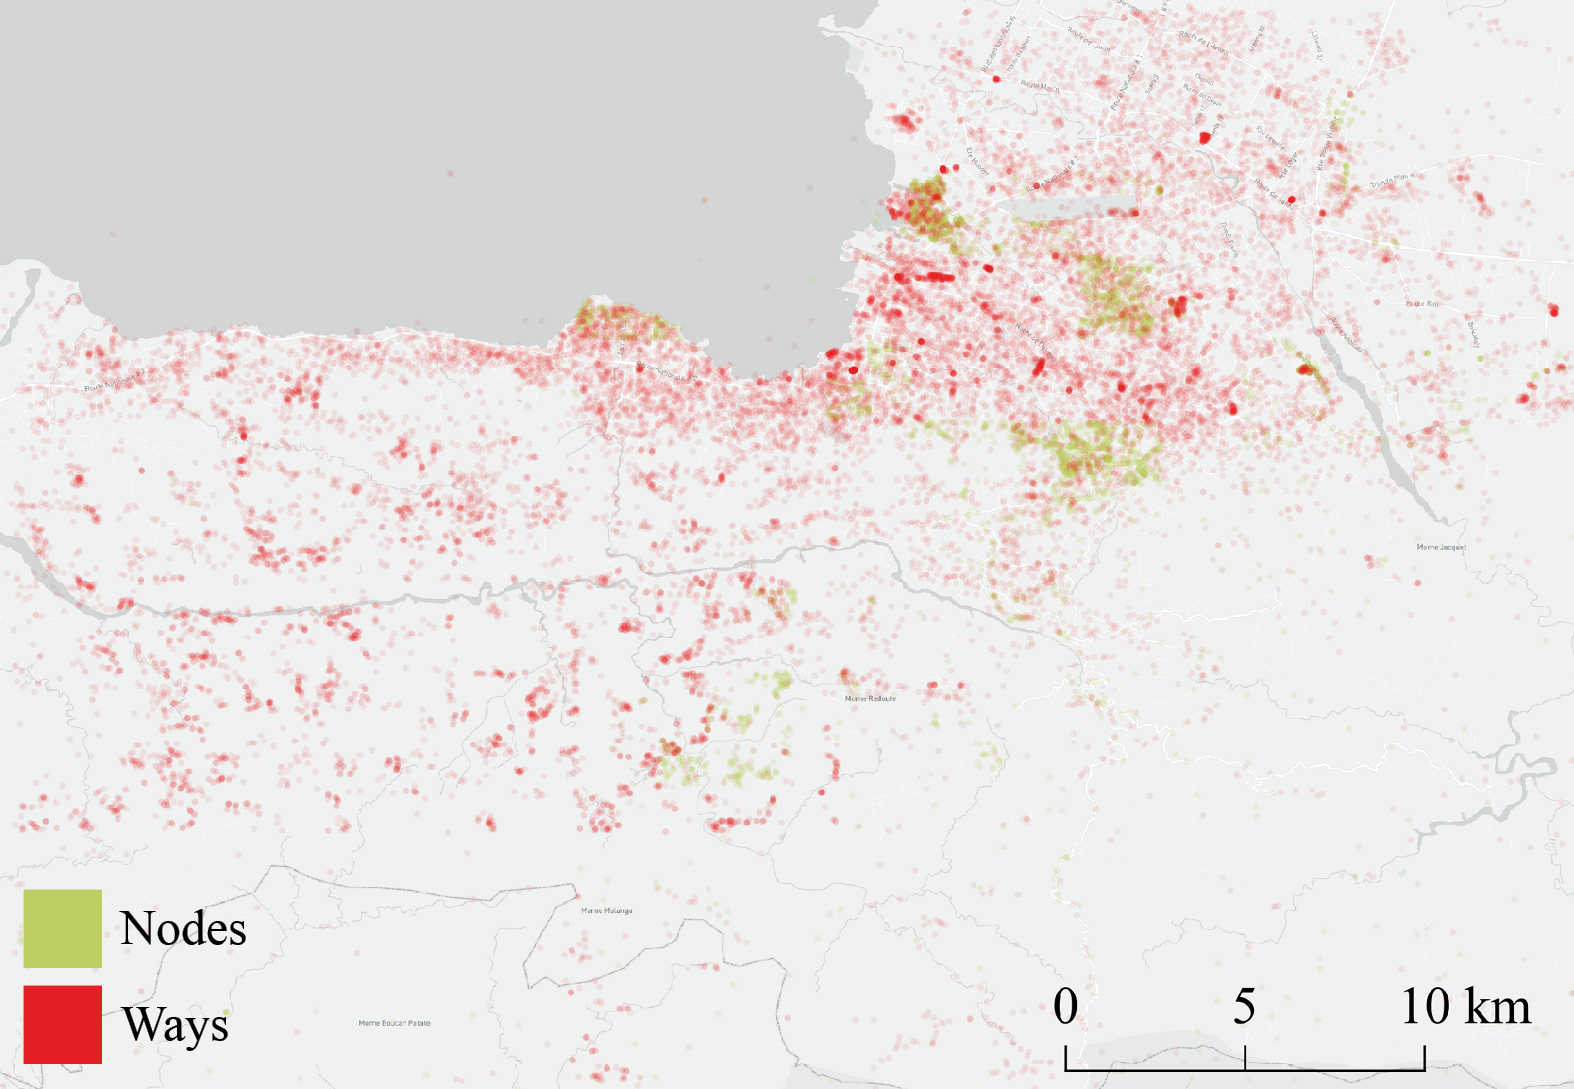
\includegraphics[width = \textwidth]{Images/pap_map.png}
    \caption[Port au Prince dot density map]{Dot density map of OSM contributions across case study area in Port au Prince} 
    \label{fig:pap} 
\end{figure}
%%%%%%%%%%%%%%%%%%%%%%%%%% 

%%%%%%%%%%%%%%%%%%%%%%%%%% Tac map 
\begin{figure}
    \centering 
    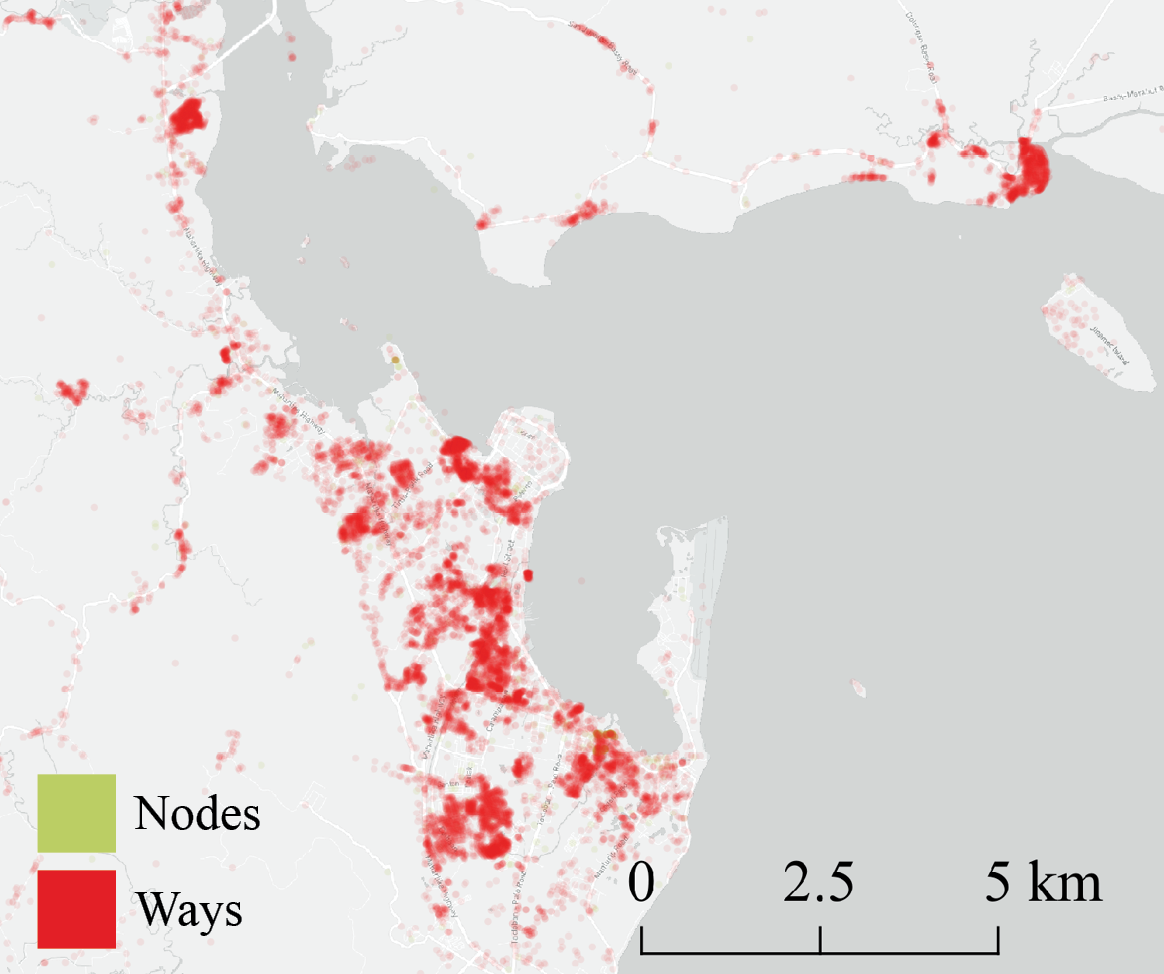
\includegraphics[width = \textwidth]{Images/tac_map.png}
    \caption[Tacloban dot density map]{Dot density map of OSM contributions across case study area in Tacloban} 
    \label{fig:tac} 
\end{figure}
%%%%%%%%%%%%%%%%%%%%%%%%%% 

\subsubsection{Tacloban, Philippines}

The Philippines was greatly impacted by a tropical cyclone, Typhoon Haiyan (or Typhoon Yolanda), on November 8, 2013. This typhoon is said to be one of the strongest ever recorded \parencite{lum_typhoon_2014}. USAID estimates that this disaster has caused over 6,000 deaths and the destruction or damage of over 1 million homes \parencite{noauthor_typhoon_2014}. The city of Tacloban was one of the areas that faced greatest impact and was thus where much relief effort was focused \parencite{lum_typhoon_2014}. Following this crisis, mapping efforts in OSM were coordinated by HOT, with high-volume, remote mapping efforts organized by the newly developed Tasking Manager \parencite{noauthor_wikiproject_2018}. \textcite{palen_success_2015} note that the mapping efforts in the Philippines were facilitated by these new tools for technical collaboration, which incorporated lessons learned from previous humanitarian mapping efforts, such as in Haiti. Details from the OSM Wiki page indicate that most mapping efforts were focused on buildings, roads, and infrastructure damage \parencite{noauthor_wikiproject_2018}. 

%%%%%%%%%%%%%%%%%%%%%%%%%% Nep map 
\begin{figure}
    \centering 
    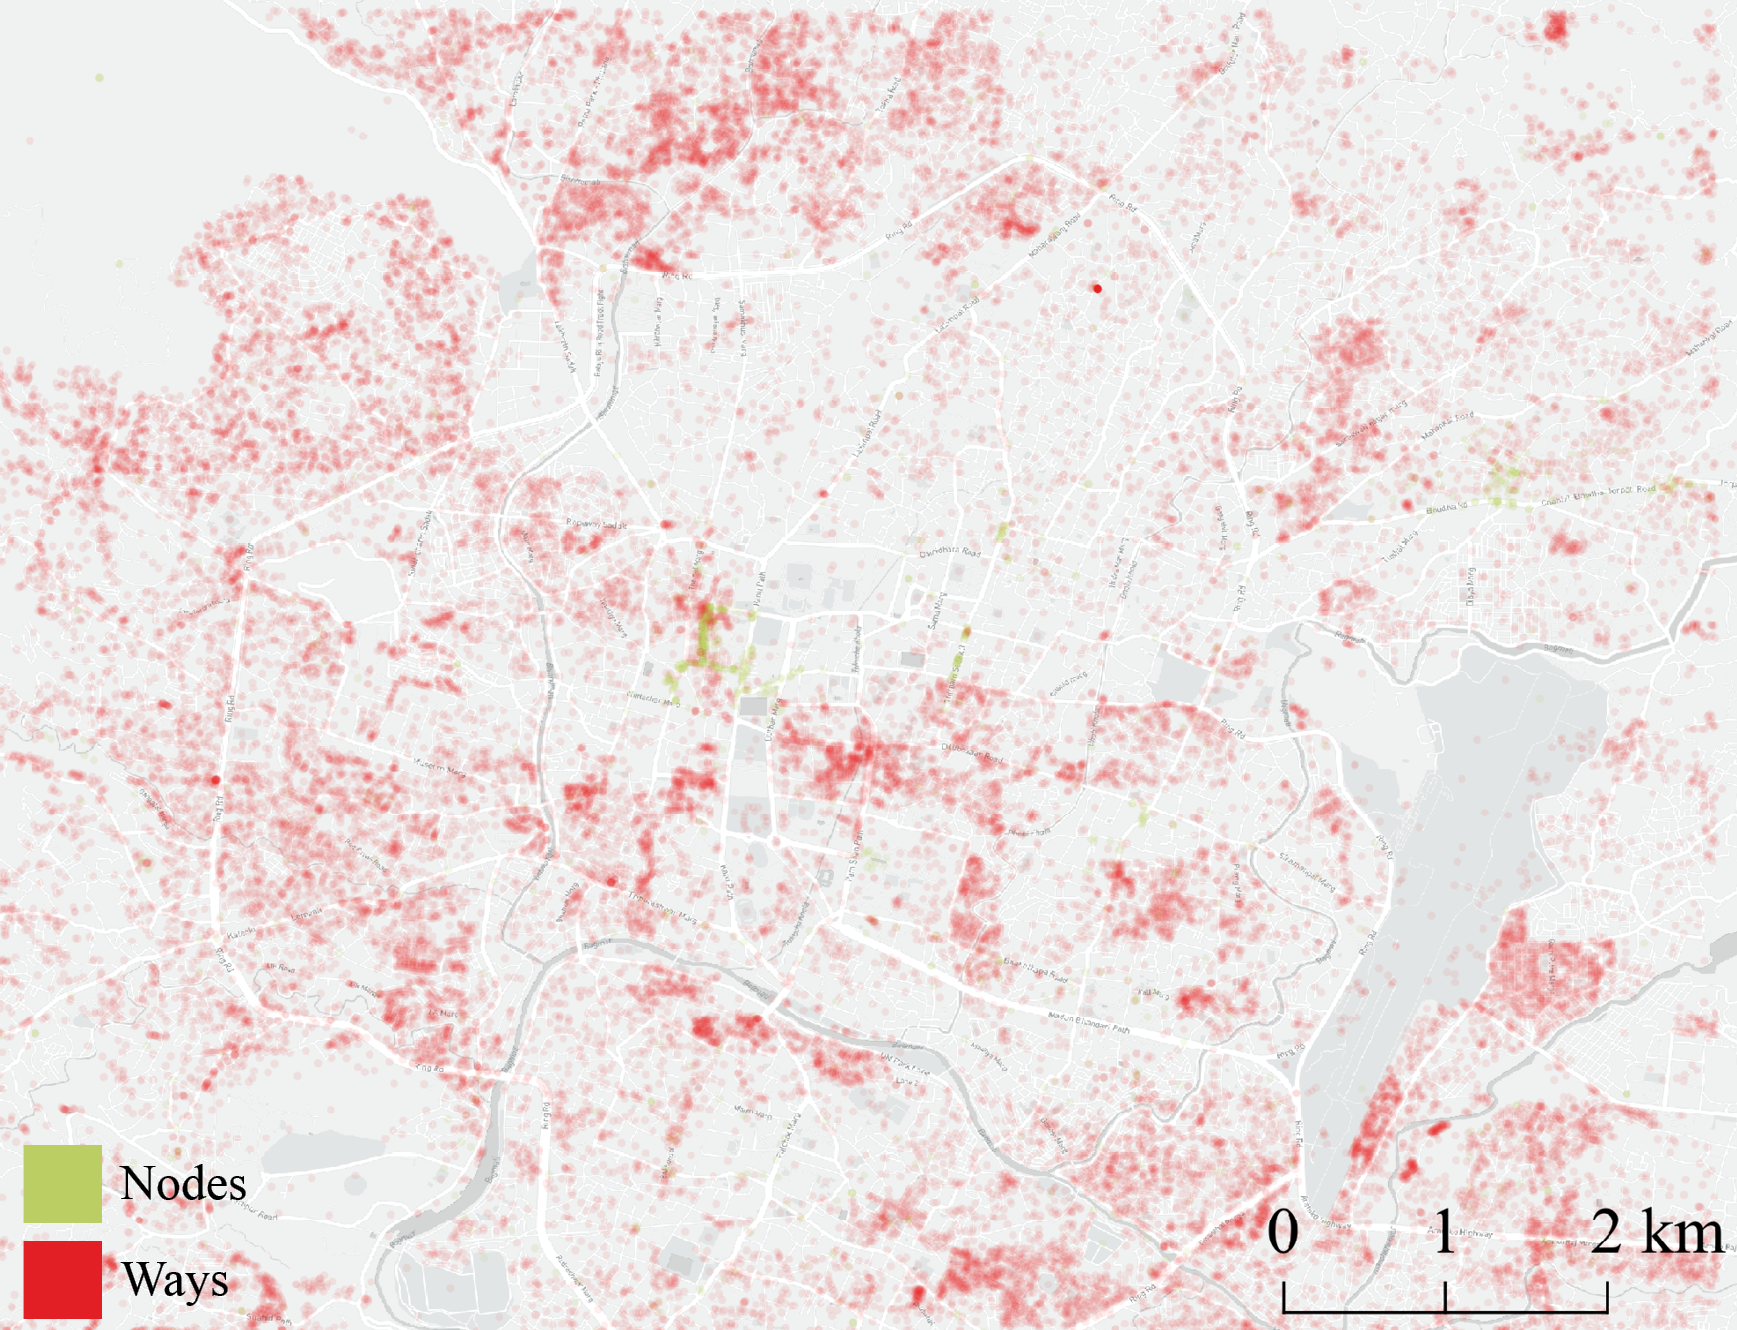
\includegraphics[width = \textwidth]{Images/nep_map.png}
    \caption[Kathmandu dot density map]{Dot density map of OSM contributions across case study area in Kathmandu} 
    \label{fig:nep} 
\end{figure}
%%%%%%%%%%%%%%%%%%%%%%%%%%

\subsubsection{Kathmandu, Nepal}

Nepal was hit with a magnitude 7.6 earthquake on April 25th, centered approximated 76 km northwest of Kathmandu, which was followed by over 300 aftershocks of over 4.0 magnitude \parencite{noauthor_nepal_2015}. It is estimated that over 9,000 people died in these disasters and over half a million homes were destroyed or damaged \parencite{noauthor_nepal_2015}. The major earthquake and its aftershocks caused further disasters such as landslides and avalanches, and exacerbated vulnerabilities to flooding in many areas \parencite{noauthor_nepal_2015}. As is described by \textcite{soden_infrastructure_2016} this crisis can be viewed as a turning point in the history of post-disaster mapping in the OSM community. Whereas in the Haiti case where HOT needed to conduct notable outreach to spread awareness of the applicability of OSM data, interviews with GIS practitioners in the field found that up-to-date OSM data came to be an 'expected resource' in Nepal \parencite[p. 2801]{soden_infrastructure_2016}


\subsubsection{Bangui, Central African Republic}

Violence and instability in CAR mounted in March 2013 when the Seleka rebel group seized the capital city, Bangui \parencite{noauthor_violence_2020}. This event launched a humanitarian mapping activation that aimed to provide baseline geospatial data for the country \parencite{noauthor_wikiproject_2020-1}. Mapping the country's road network was a priority of this activation, as well as mapping affected cities and towns, as idenfitied by local humanitarian stakeholders \parencite{noauthor_wikiproject_2020-1}. UNICEF data for health facilities, water points, and schools was also imported as part of this activation \parencite{noauthor_wikiproject_2020-1}.

%%%%%%%%%%%%%%%%%%%%%%%%%% Car map 
\begin{figure}
    \centering 
    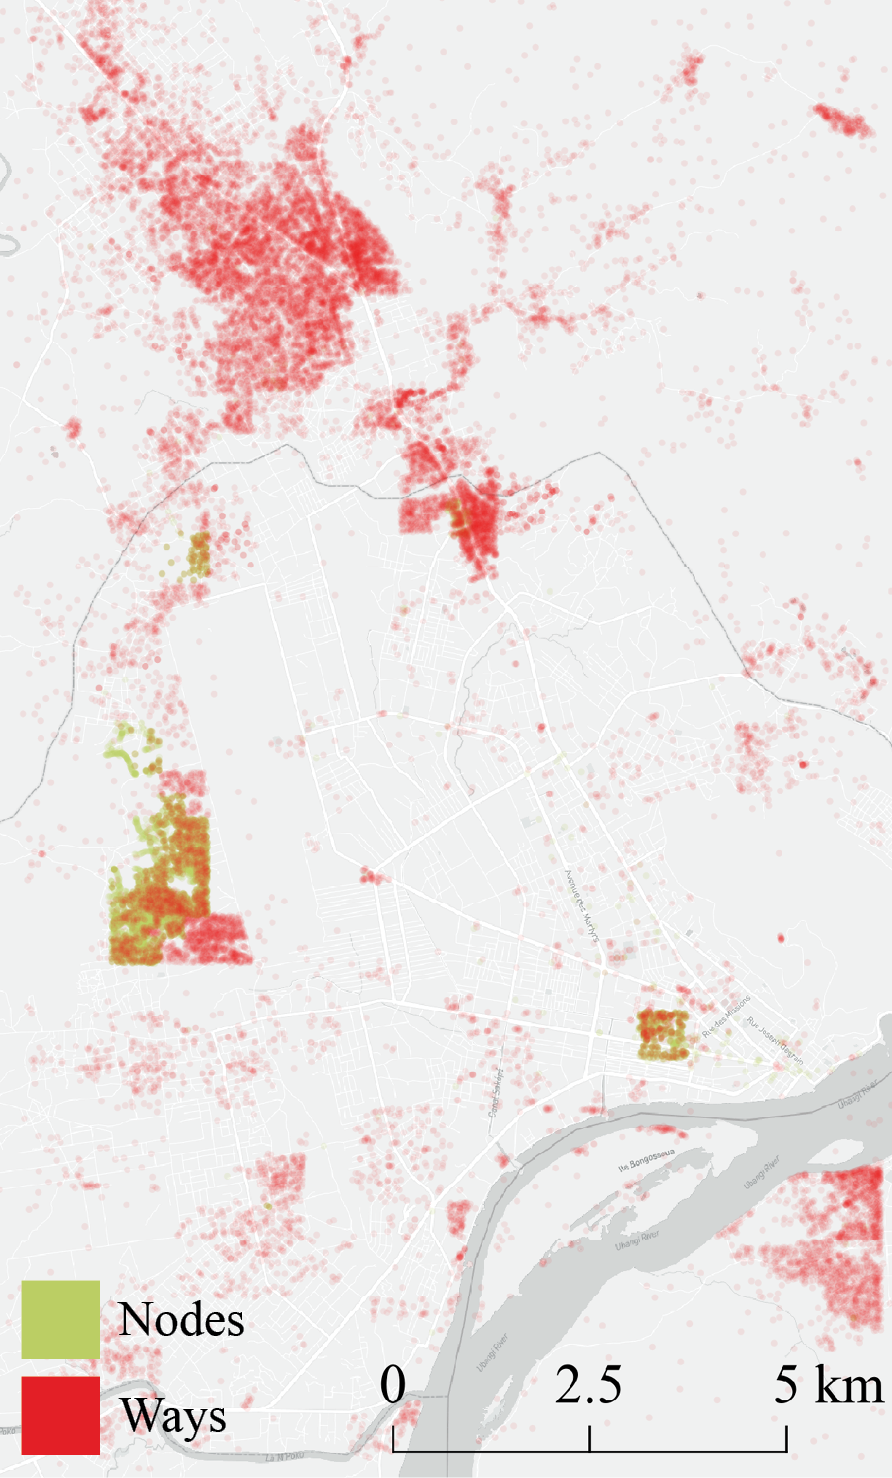
\includegraphics[width = \textwidth]{Images/ban_map.png}
    \caption[Bangui dot density map]{Dot density map of OSM contributions across case study area in Bangui} 
    \label{fig:car} 
\end{figure}
%%%%%%%%%%%%%%%%%%%%%%%%%% 

\subsubsection{Heidelberg, Germany}

%%%%%%%%%%%%%%%%%%%%%%%%%% Hed map 
\begin{figure}
    \centering 
    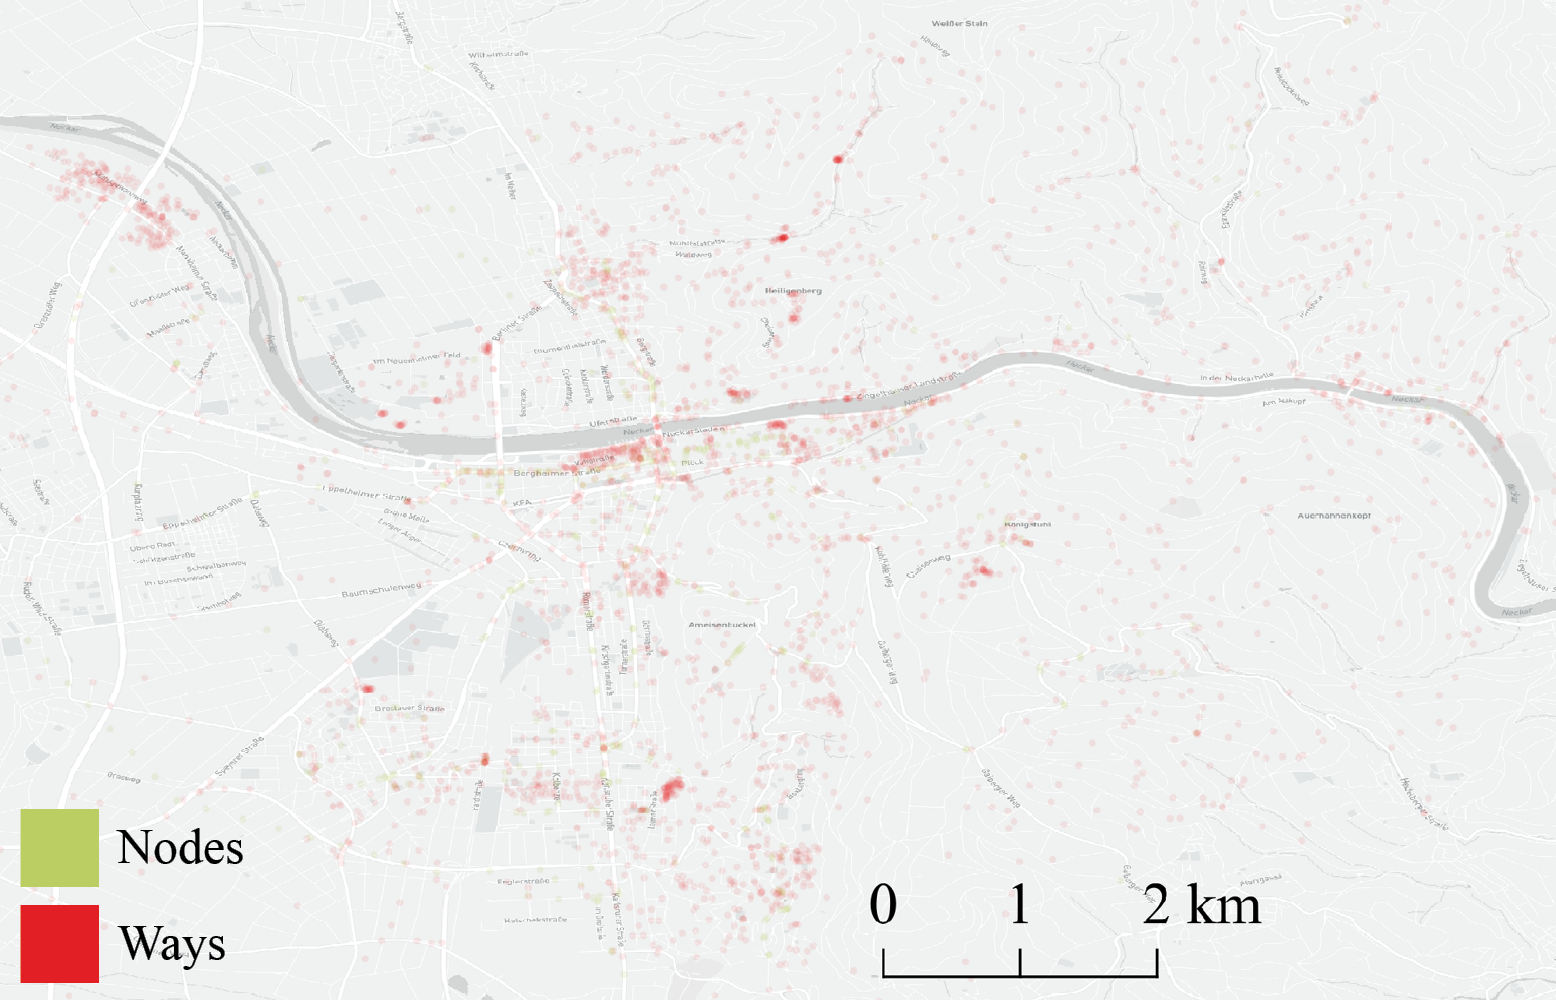
\includegraphics[width = \textwidth]{Images/hed_map.png}
    \caption[Heidelberg dot density map]{Dot density map of OSM contributions across case study area in Heidelberg} 
    \label{fig:hed} 
\end{figure}
%%%%%%%%%%%%%%%%%%%%%%%%%% 

\subsection{Dynamics of data production over time}


The dynamics of contributing patterns for each case study are further demonstrated in Figure \ref{fig:time}, which shows the daily magnitude of contributions for each mapping activation. The activations in Tacloban, Port au Prince, and Kathmandu exhibit the clear ‘event-style’ as described by \textcite{dittus_mass_2017}, whereby mapping activity is front-loaded and decays quickly after the beginning of the activation. The magnitude of early mapping efforts in Tacloban and Kathmandu, shown by the burstiness values from Table \ref{tab:summary} and the size of the peaks in Figure \ref{fig:time}, set these cases apart from others. Whereas the activation in Bangui and the Heidelberg reference show a ‘mission-style’ where activity is more evenly sustained over a longer period of time. 

%%%%%%%%%%%%%%%%%%%%%%%%%% Over time image 
\begin{figure} % opens the figure environment. the '[H]' forces the image to be Here
    \centering % puts the image in the horizontal centre of the page
    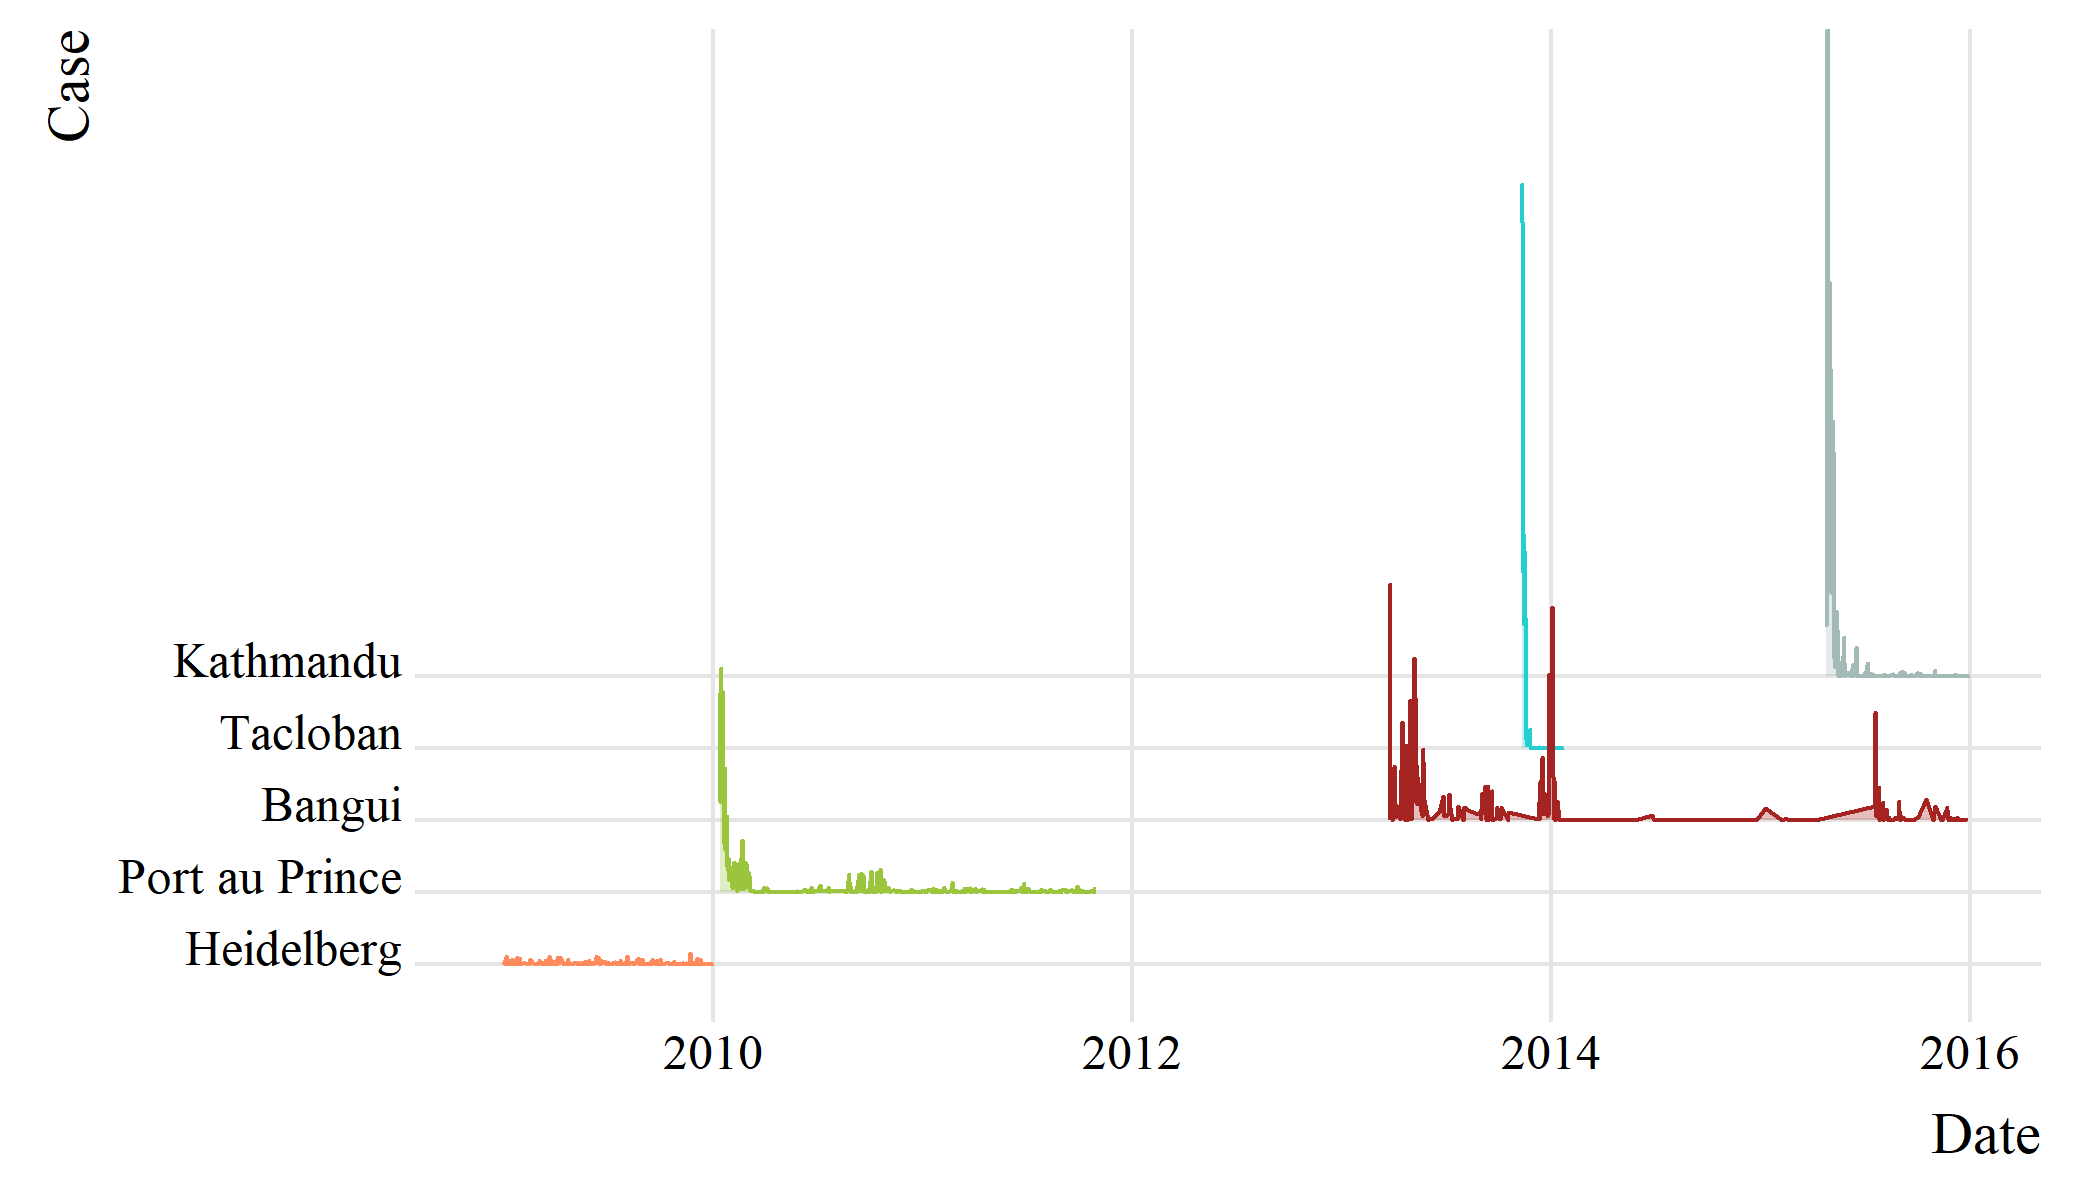
\includegraphics[width = \textwidth]{Images/overtime.png} %this tells latex what graphics to include. 
    \caption{Daily volume of OSM contributions throughout extent of each mapping activation. } % this prints the caption below the figure
    \label{fig:time} % this internally labels the figure for future referencing.
\end{figure}
%%%%%%%%%%%%%%%%%%%%%%%%%% 

Further differences between the two mapping activation styles are shown in Figure \ref{fig:scatter}, where we see that the ‘event-style’ activations have a stronger relationship between the number of daily contributors and contributions.  In all cases, however, the relationship between daily contributor volume and daily contribution volume is statistically significant. Heidelberg and Bangui, the two ‘mission-style’ activations, have a notably shorter range of daily unique contributors (no more than 10 in a day), while activations such as that in Kathmandu have reached over 150 unique contributors in a day. 

Both Figures \ref{fig:time} and \ref{fig:scatter} show a clear difference in the daily volume of data contributed between the Heidelberg reference and the humanitarian activations.  Daily contribution volume in Heidelberg during this time barely exceed 100 new entities, while humanitarian activations such as those in Tacloban and Kathmandu reach over 4,000 and 6,000 new entities in a day, respectively, at their peaks. 

%%%%%%%%%%%%%%%%%%%%%%%%%% Scatter image
\begin{figure}[H] % opens the figure environment. the '[H]' forces the image to be Here
    \centering % puts the image in the horizontal centre of the page
    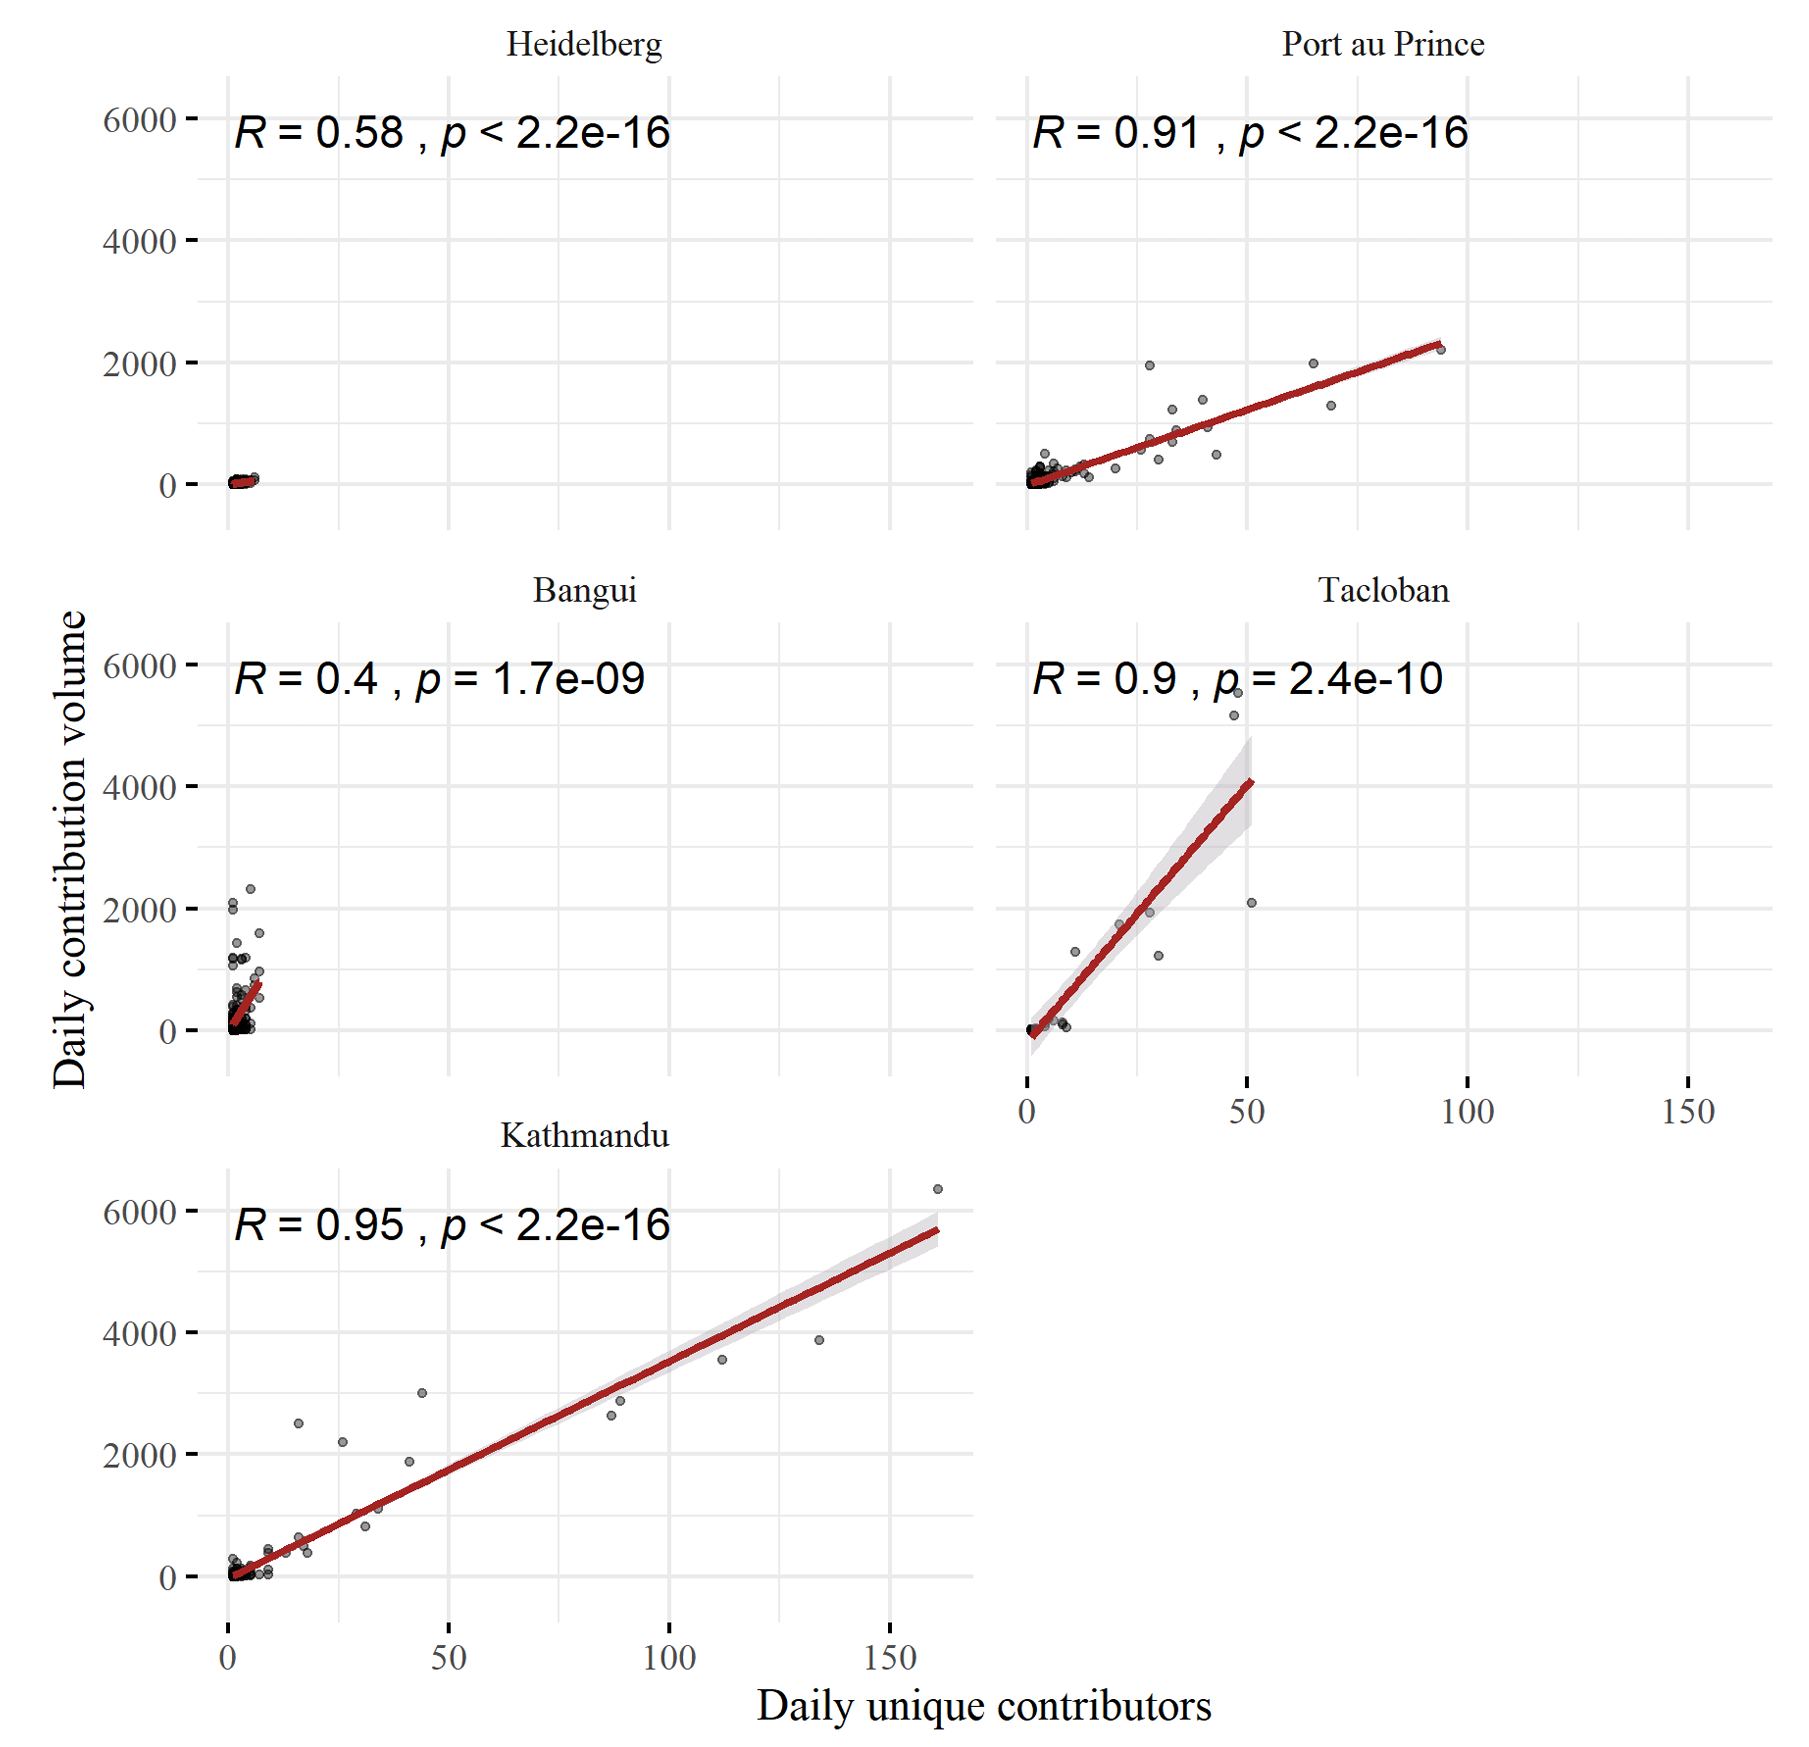
\includegraphics[width = \textwidth]{Images/scatter.png} %this tells latex what graphics to include. 
    \caption{Scatterplots of daily unique contributors against daily contribution volume (in number of contributions) for each mapping activation.} % this prints the caption below the figure
    \label{fig:scatter} % this internally labels the figure for future referencing.
\end{figure}
%%%%%%%%%%%%%%%%%%%%%%%%%% 

%%%%%%%%%%%%%%%%%%%%%%%%%% Scatter image
\begin{figure}[H] % opens the figure environment. the '[H]' forces the image to be Here
    \centering % puts the image in the horizontal centre of the page
    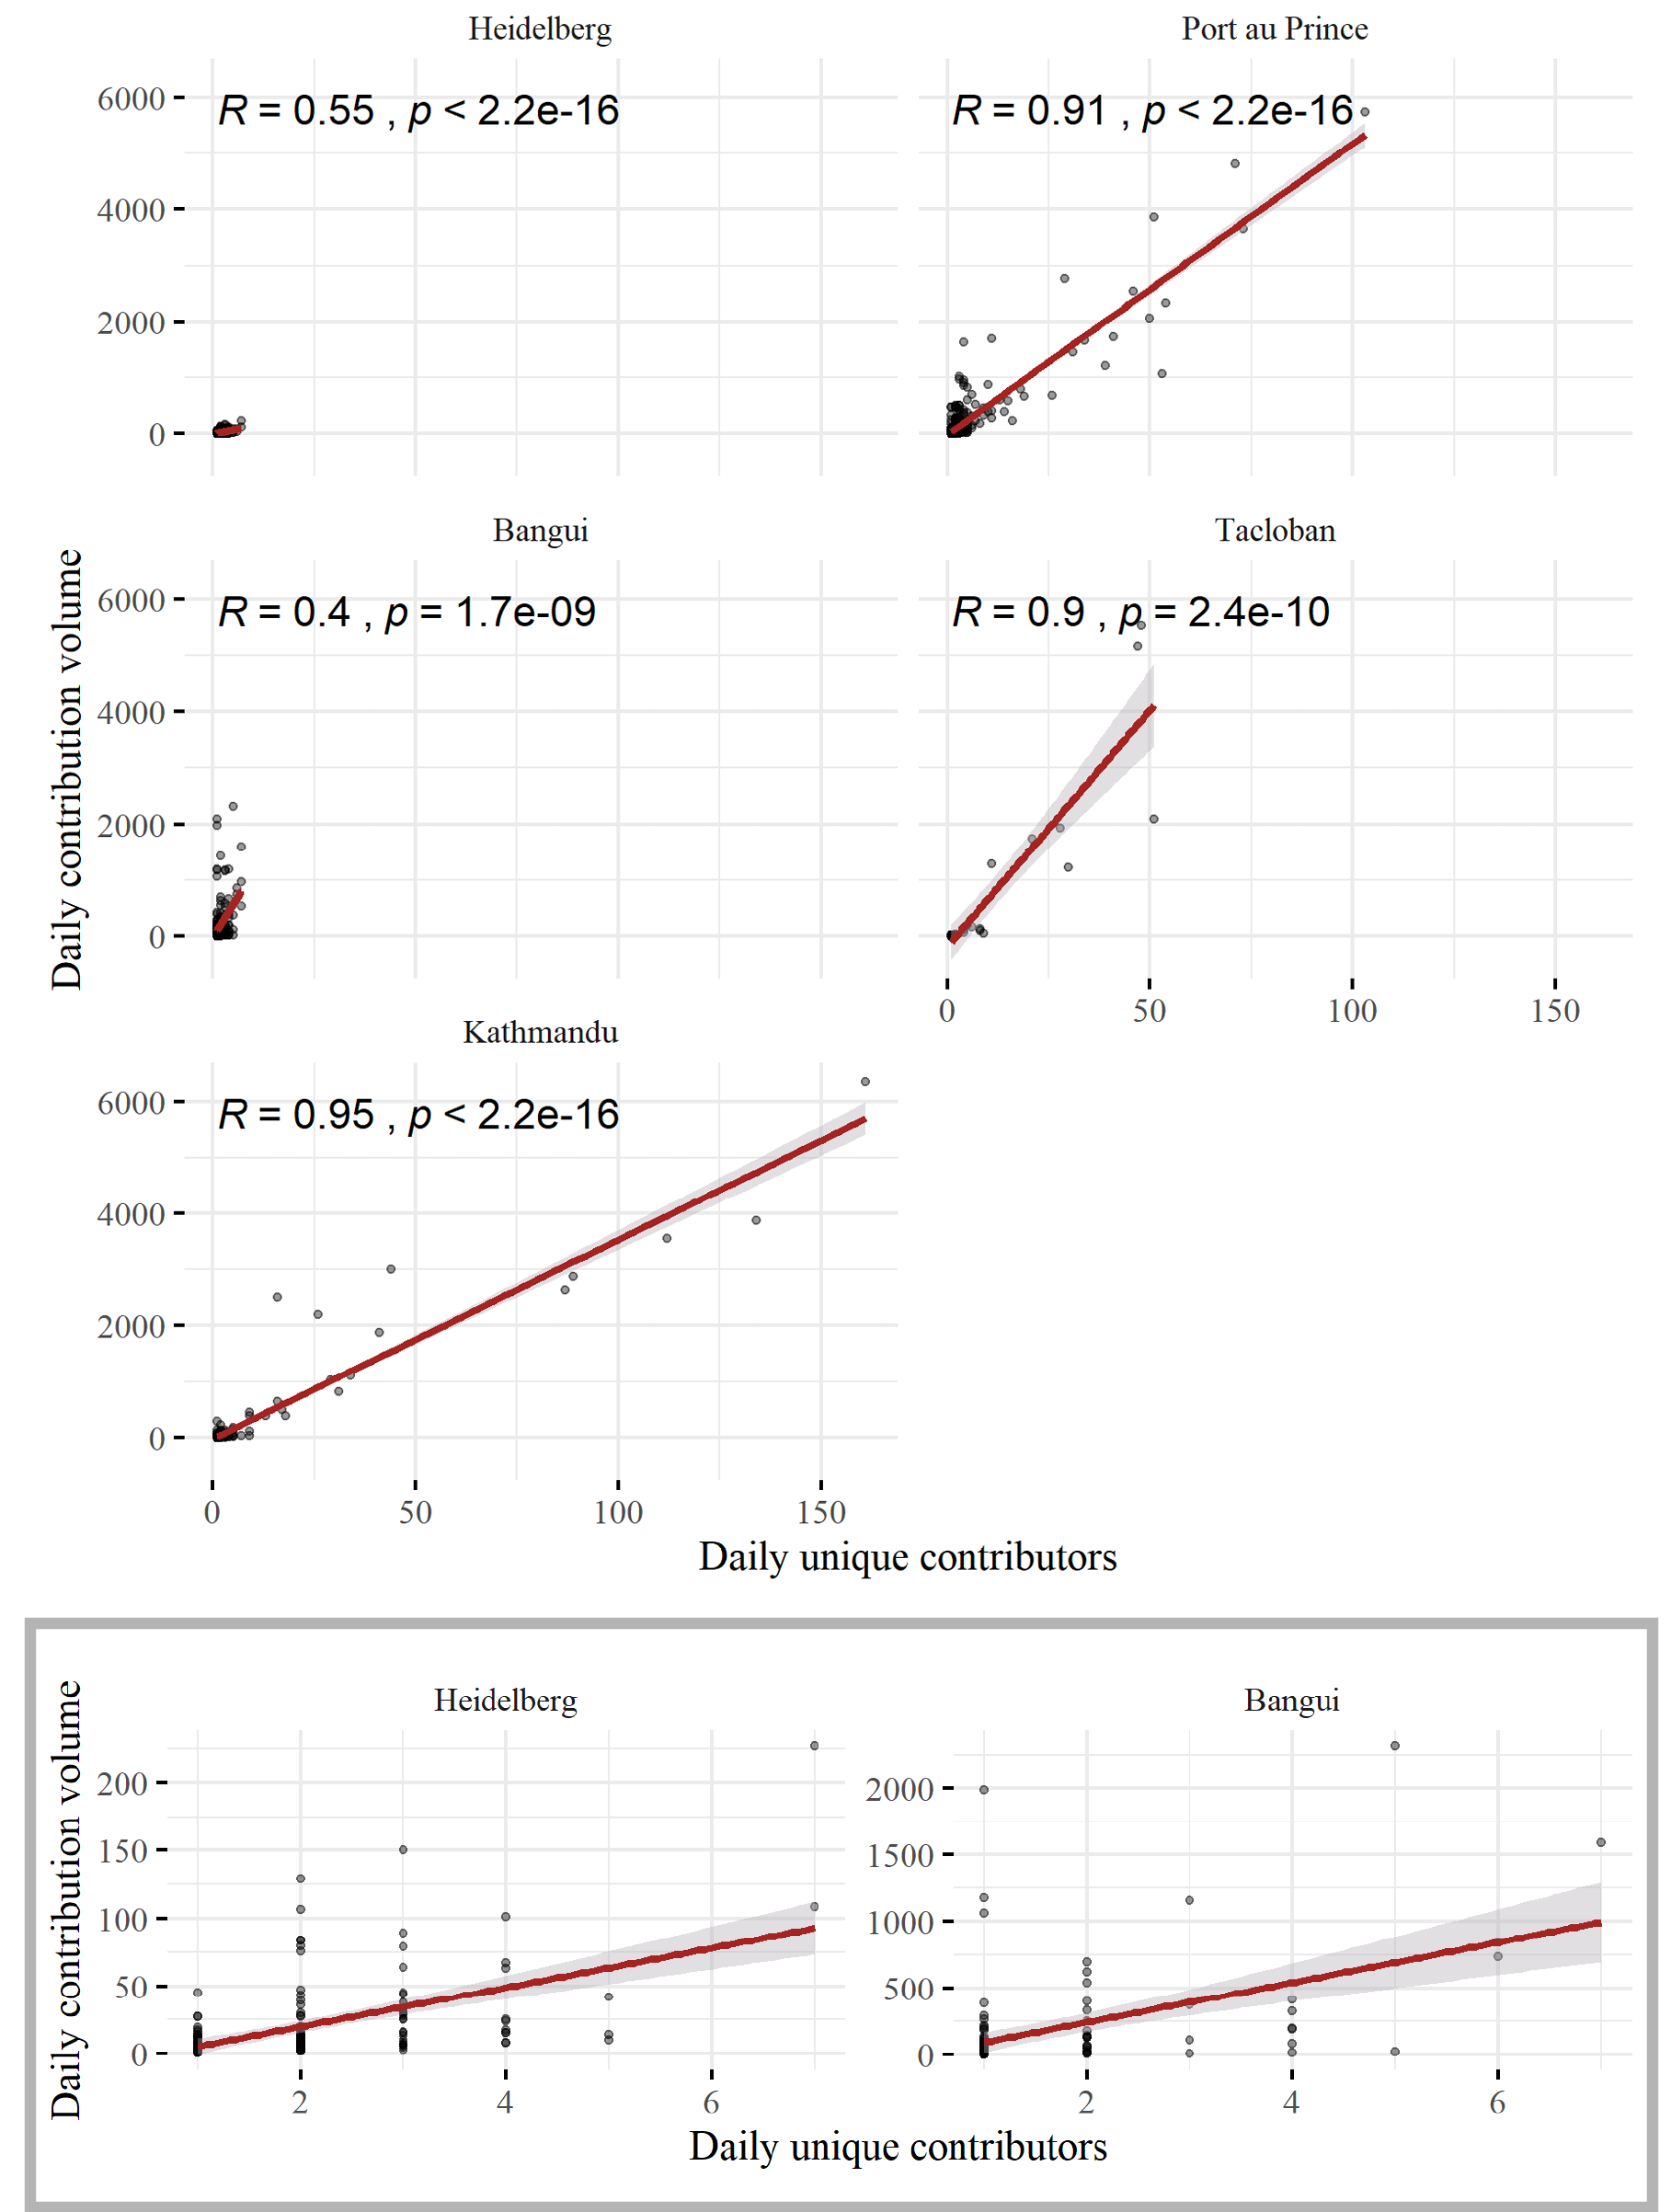
\includegraphics[width = \textwidth]{Images/scatter_inset.png} %this tells latex what graphics to include. 
    \caption{Scatterplots of daily unique contributors against daily contribution volume (in number of contributions) for each mapping activation.} % this prints the caption below the figure
    \label{fig:scatter_inset} % this internally labels the figure for future referencing.
\end{figure}
%%%%%%%%%%%%%%%%%%%%%%%%%% 

\subsection{Types of entities produced and information sources}

Table \ref{tab:tags}, below, provides insight into the type of data that is contributed in each mapping activation. We see similarities across all cases as the ‘building’, ‘highway’, and ‘source’ tags are frequently occurring in each. The humanitarian activations show crisis-specific tags, such as ‘typhoon:damage’ and ‘damage:event’. Mapping activities in Heidelberg may be more matured than in the humanitarian activations, as indicated by the presence of address tags. 

Table \ref{tab:sources} provides insight into the data sources for each mapping activation. For the humanitarian cases, we see that a notable proportion of the data was generated from satellite imagery (eg. Bing or Worldview), suggesting that many of the contributors are remotely located. Very little of the Heidelberg data has been tagged with a source, however none of the sources listed are from satellite imagery, so we can perhaps infer that much of this data was added by local contributors. 

%%%%%%%%%%%%%%%%%%%%%%%%%% TABLE - tags 
\begin{table}
\centering
\caption{Top five most frequently occurring tag keys across each case study. Keys highlighted in grey appear across at least 4/5 case studies.}
\label{tab:tags}
\begin{tabular}{@{} llll @{}} 
\toprule
Port au Prince                               &                  & Tacloban                                     &                   \\ 
\midrule
\textit{key}                                 & \textit{percent} & \textit{key}                                 & \textit{percent}  \\
{\cellcolor[rgb]{0.875,0.875,0.875}}source   & \Chart{0.76}             & {\cellcolor[rgb]{0.875,0.875,0.875}}building & \Chart{0.89}              \\
{\cellcolor[rgb]{0.875,0.875,0.875}}highway  & \Chart{0.39}             & {\cellcolor[rgb]{0.875,0.875,0.875}}source   & \Chart{0.27}              \\
{\cellcolor[rgb]{0.875,0.875,0.875}}building & \Chart{0.31}             & typhoon:damage                               & \Chart{0.11}                \\
attribute\_source\_date                      & \Chart{0.12}             & {\cellcolor[rgb]{0.875,0.875,0.875}}highway  & \Chart{0.27}               \\
name                                         & \Chart{0.11}             & typhoon:damaged                              & \Chart{0.15}               \\ 
\toprule
Bangui                                       &                  & Kathmandu                                    &                   \\ 
\midrule
\textit{key}                                 & \textit{percent} & \textit{key}                                 & \textit{percent}  \\
{\cellcolor[rgb]{0.875,0.875,0.875}}building & \Chart{0.58}             & {\cellcolor[rgb]{0.875,0.875,0.875}}building & \Chart{0.74}              \\
{\cellcolor[rgb]{0.875,0.875,0.875}}source   & \Chart{0.35}               & {\cellcolor[rgb]{0.875,0.875,0.875}}source   & \Chart{0.24}              \\
{\cellcolor[rgb]{0.875,0.875,0.875}}highway  & \Chart{0.11}             & idp:camp\_site                               & \Chart{0.14}              \\
source:date                                  & \Chart{0.06}              & damage:event                                 & \Chart{0.13}              \\
project:eurosha\_2012                        & \Chart{0.06}              & {\cellcolor[rgb]{0.875,0.875,0.875}}highway  & \Chart{0.04}               \\ 
\toprule
Heidelberg                                   &                  &                                              &                   \\ 
\midrule
\textit{key}                                 & \textit{percent} &                                              &                   \\
{\cellcolor[rgb]{0.875,0.875,0.875}}highway  & \Chart{0.70}             &                                              &                   \\
name                                         & \Chart{0.26}               &                                              &                   \\
tracktype                                    & \Chart{0.15}             &                                              &                   \\
created\_by                                  & \Chart{0.15}             &                                              &                   \\
amenity                                      & \Chart{0.09}              &                                              &     \\
\bottomrule
\end{tabular}
\end{table}
%%%%%%%%%%%%%%%%%%%%%%%%%%

%%%%%%%%%%%%%%%%%%%%%%%%%% TABLE - sources
\begin{table}
\centering
\caption{Top five most frequently occurring source values across each case study. }
\label{tab:sources}
\begin{tabular}{llll} 
\toprule
Port au Prince                                                                                                                    &                  & Tacloban                                                                                    &                   \\ 
\midrule
\textit{source}                                                                                                                   & \textit{percent} & \textit{source}                                                                             & \textit{percent}  \\
geoeye                                                                                                                            & \Chart{0.230}            & bing                                                                                        & \Chart{0.131}              \\
google; 2010-01-21                                                                                                                & \Chart{0.150}            & \begin{tabular}[c]{@{}l@{}}Worldview-2; \\digitalglobe;\\nextview;\\2013/11/09\end{tabular} & \Chart{0.100}              \\
yahoo                                                                                                                             & \Chart{0.043}             & bing; 2010-11                                                                               & \Chart{0.018}              \\
NA                                                                                                                                & \Chart{0.042}             & gsi/kiban 2500; naro                                                                        & \Chart{0.004}              \\
google 2010-01-17                                                                                                                 & \Chart{0.033}             & \begin{tabular}[c]{@{}l@{}}hot task 355 \\image (arcgis)\end{tabular}                       & \Chart{0.021}              \\ 
\toprule
Bangui                                                                                                                            &                  & Kathmandu                                                                                   &                   \\ 
\midrule
\textit{source}                                                                                                                   & \textit{percent} & \textit{source}                                                                             & \textit{percent}  \\
bing                                                                                                                              & \Chart{0.186}            & \begin{tabular}[c]{@{}l@{}}pleiades 2015-04-27;\\cnes;airbus ds\end{tabular}                & \Chart{0.135}              \\
bing 2012                                                                                                                         & \Chart{0.132}            & nextview                                                                                    & \Chart{0.079}              \\
worldview1                                                                                                                        & \Chart{0.015}             & bing                                                                                        & \Chart{0.014}              \\
bing et hotosm                                                                                                                    & \Chart{0.012}             & gsimaps/std                                                                                 & \Chart{0.005}              \\
NA                                                                                                                                & \Chart{0.003}             & bing imagery                                                                                & \Chart{0.001}              \\ 
\toprule
Heidelberg                                                                                                                        &                  &                                                                                             &                   \\ 
\midrule
\textit{source}                                                                                                                   & \textit{percent} &                                                                                             &                   \\
survey                                                                                                                            & \Chart{0.002}             &                                                                                             &                   \\
\begin{tabular}[c]{@{}l@{}}http://wiki.openstreetmap\\.org/wiki/import/catalogue\\/kreisgrenzen\_deutschland\\\_2005\end{tabular} & \Chart{0.002}             &                                                                                             &                   \\
gps                                                                                                                               & \Chart{0.001}             &                                                                                             &                   \\
estimation                                                                                                                        & \Chart{0.001}             &                                                                                             &                   \\
rectified\_map:837                                                                                                                & \Chart{0.001}              &                                                                                             &       \\
\bottomrule
\end{tabular}
\end{table}
%%%%%%%%%%%%%%%%%%%%%%%%%% 

\section{Prevalence of data maintenance}

Following a review of the characteristics of data production across case studies, we now present results that provide insight into the trajectory of this data over time. Specifically, these results indicate the prevalence of data maintenance efforts in the years following each mapping activation. 

%%%%%%%%%%%%%%%%%%%%%%%%%% Tot maintenance
\begin{figure} % opens the figure environment. the '[H]' forces the image to be Here
    \centering % puts the image in the horizontal centre of the page
    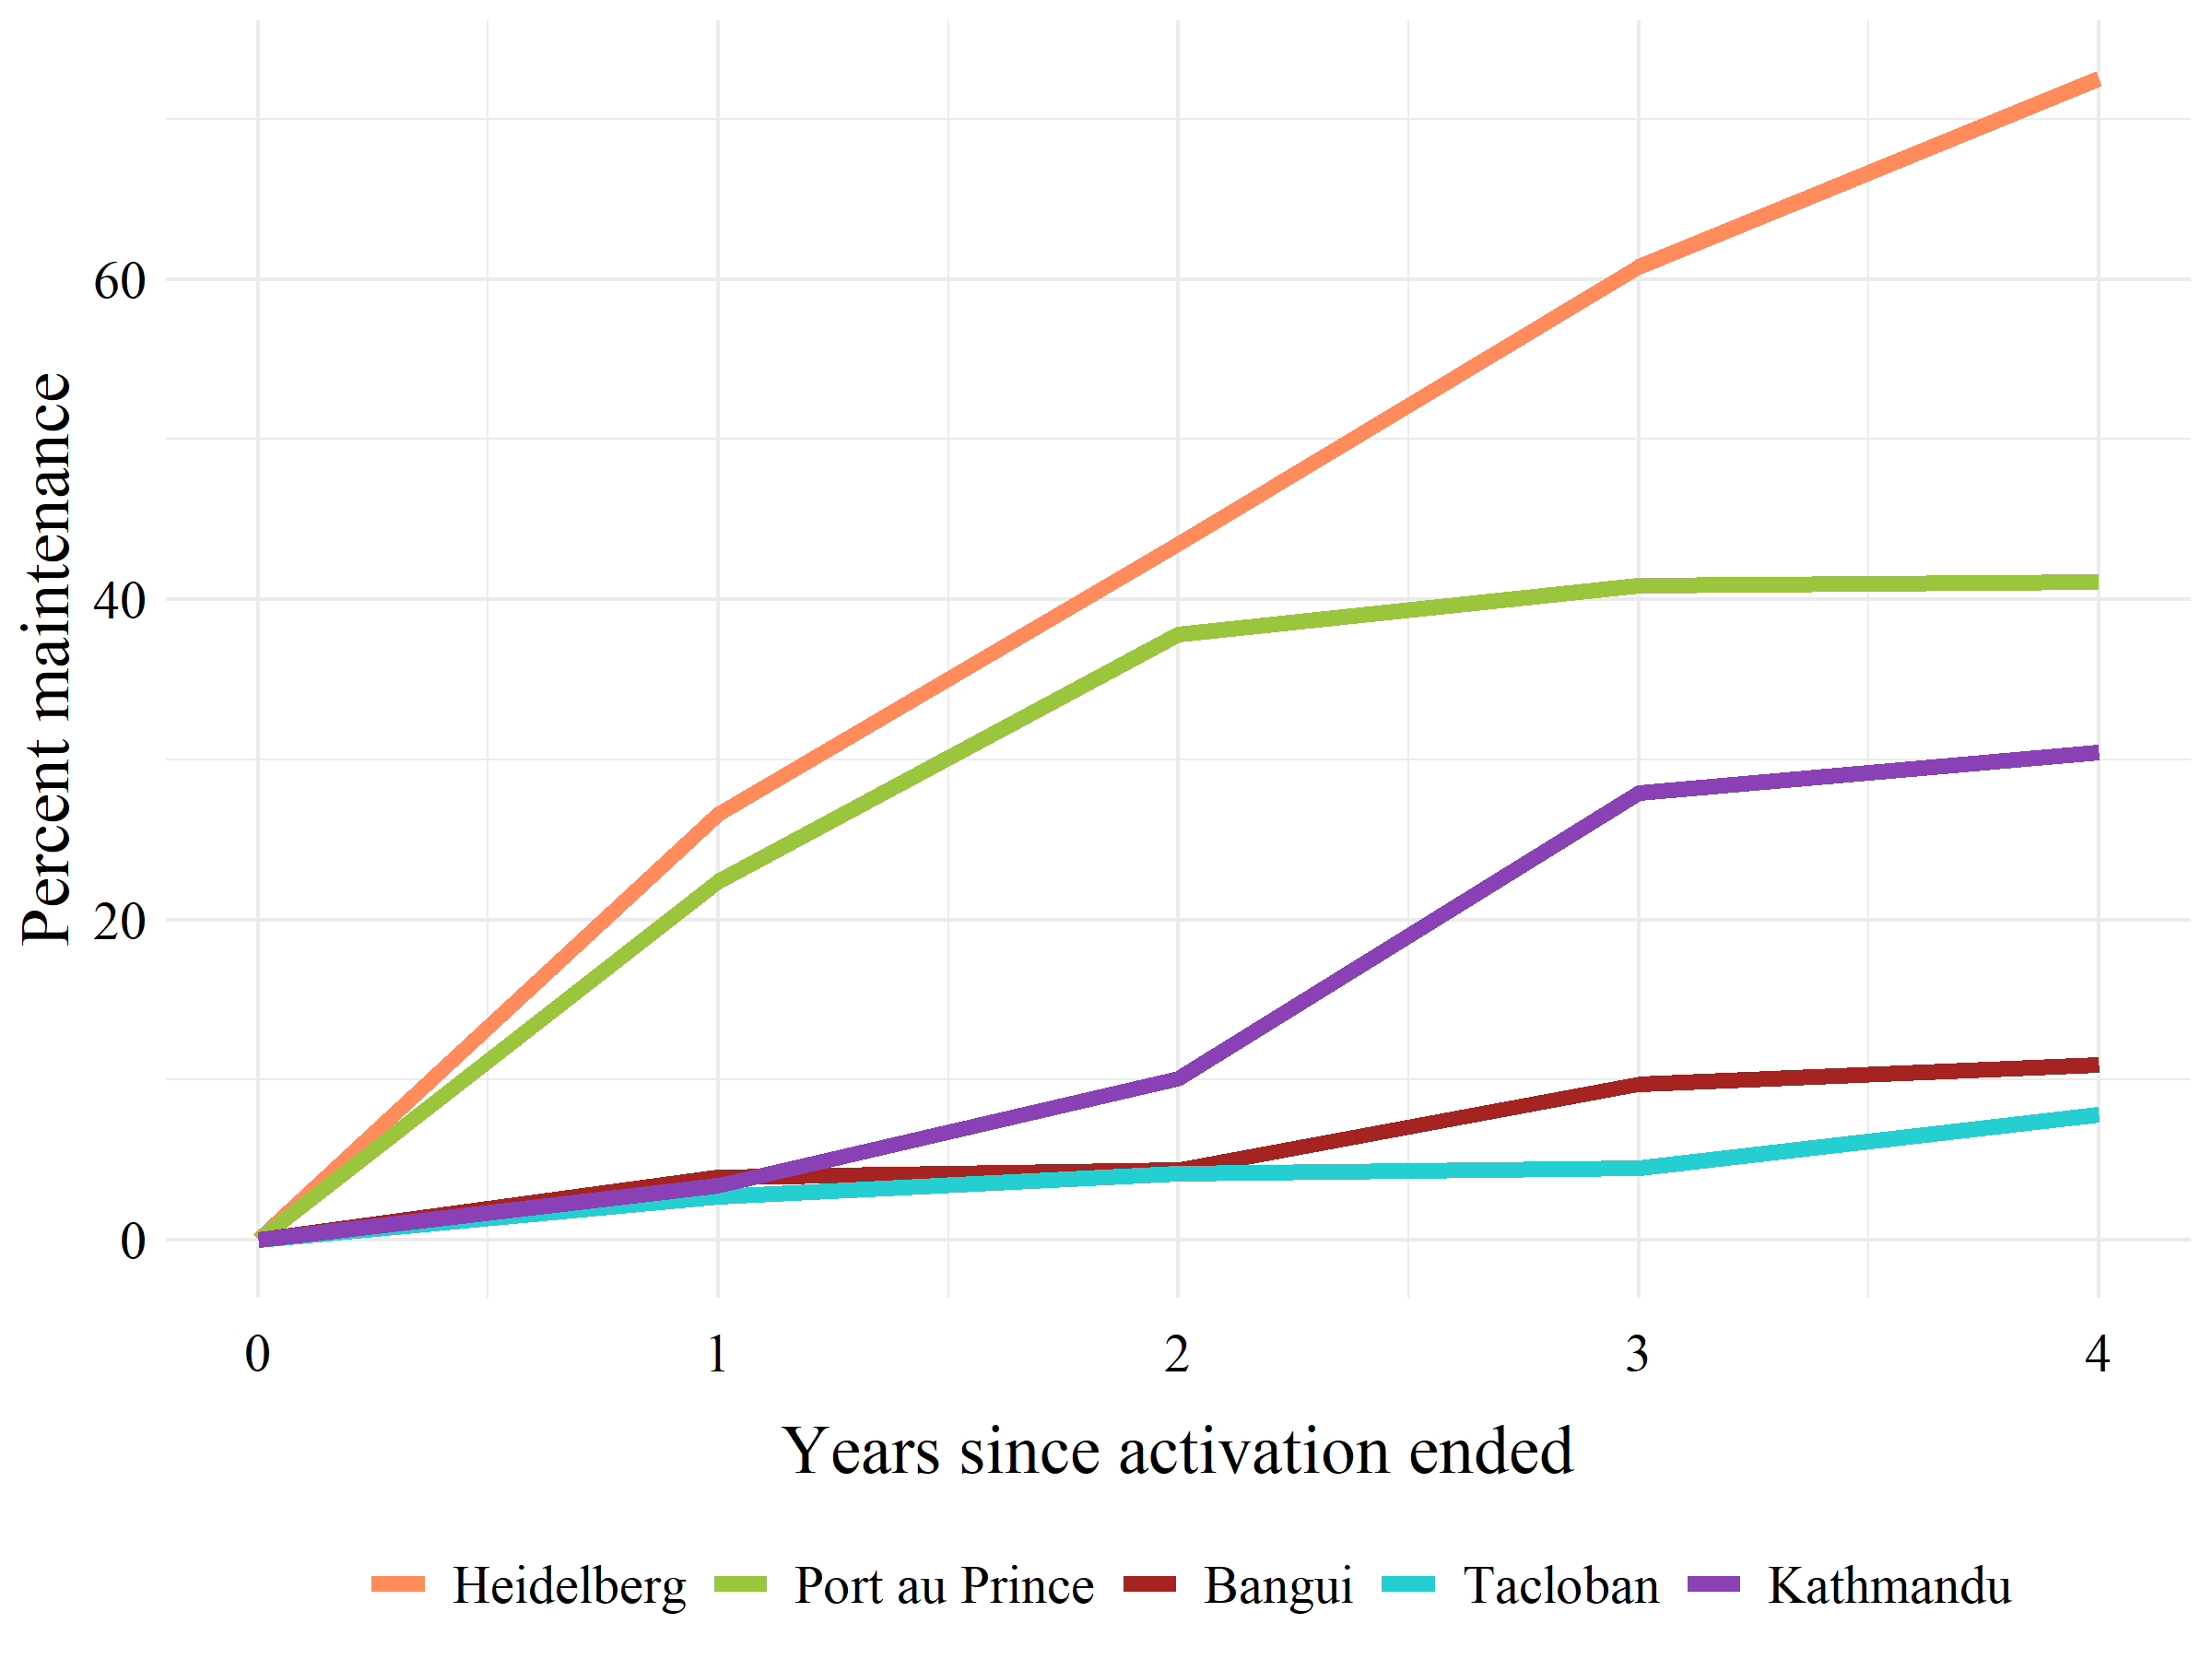
\includegraphics[width = \textwidth]{Images/totmaint.png} %this tells latex what graphics to include. 
    \caption{Cumulative percentage of maintained data (deleted or modified at least once) in years following end of mapping activation} % this prints the caption below the figure
    \label{fig:tot} % this internally labels the figure for future referencing.
\end{figure}
%%%%%%%%%%%%%%%%%%%%%%%%%% 

Figure \ref{fig:tot}, above, provides an initial look at the prevalence of data maintenance in each case study. This figure shows the cumulative percentage of entities, created during the mapping activation period, that have been modified at least once in the years after the activation has ended. We note that this and all subsequent figures include entity deletion within the definition of maintenance. 

We see that the reference case study, Heidelberg, has a significantly higher prevalence of data maintenance, as over 70\% of this data has been modified or deleted in the four years after it was originally created. Among the humanitarian case studies, the Port au Prince and Kathmandu activations stand out for both reaching above 30\% maintenance by the end if this four-year period. The other humanitarian case studies in Tacloban and Bangui only reach approximately 10\% maintenance during this time. Figure \ref{fig:tot} also shows how the rate of maintenance in Heidelberg appears to be approximately consistent during this time period, while maintenance efforts in the humanitarian case studies have plateaued in the fourth year after the activation has ended. Maintenance efforts in Kathmandu increased notably in the third year after the activation ended.

%%%%%%%%%%%%%%%%%%%%%%%%%% Distribution of maintenance
\begin{figure} % opens the figure environment. the '[H]' forces the image to be Here
    \centering % puts the image in the horizontal centre of the page
    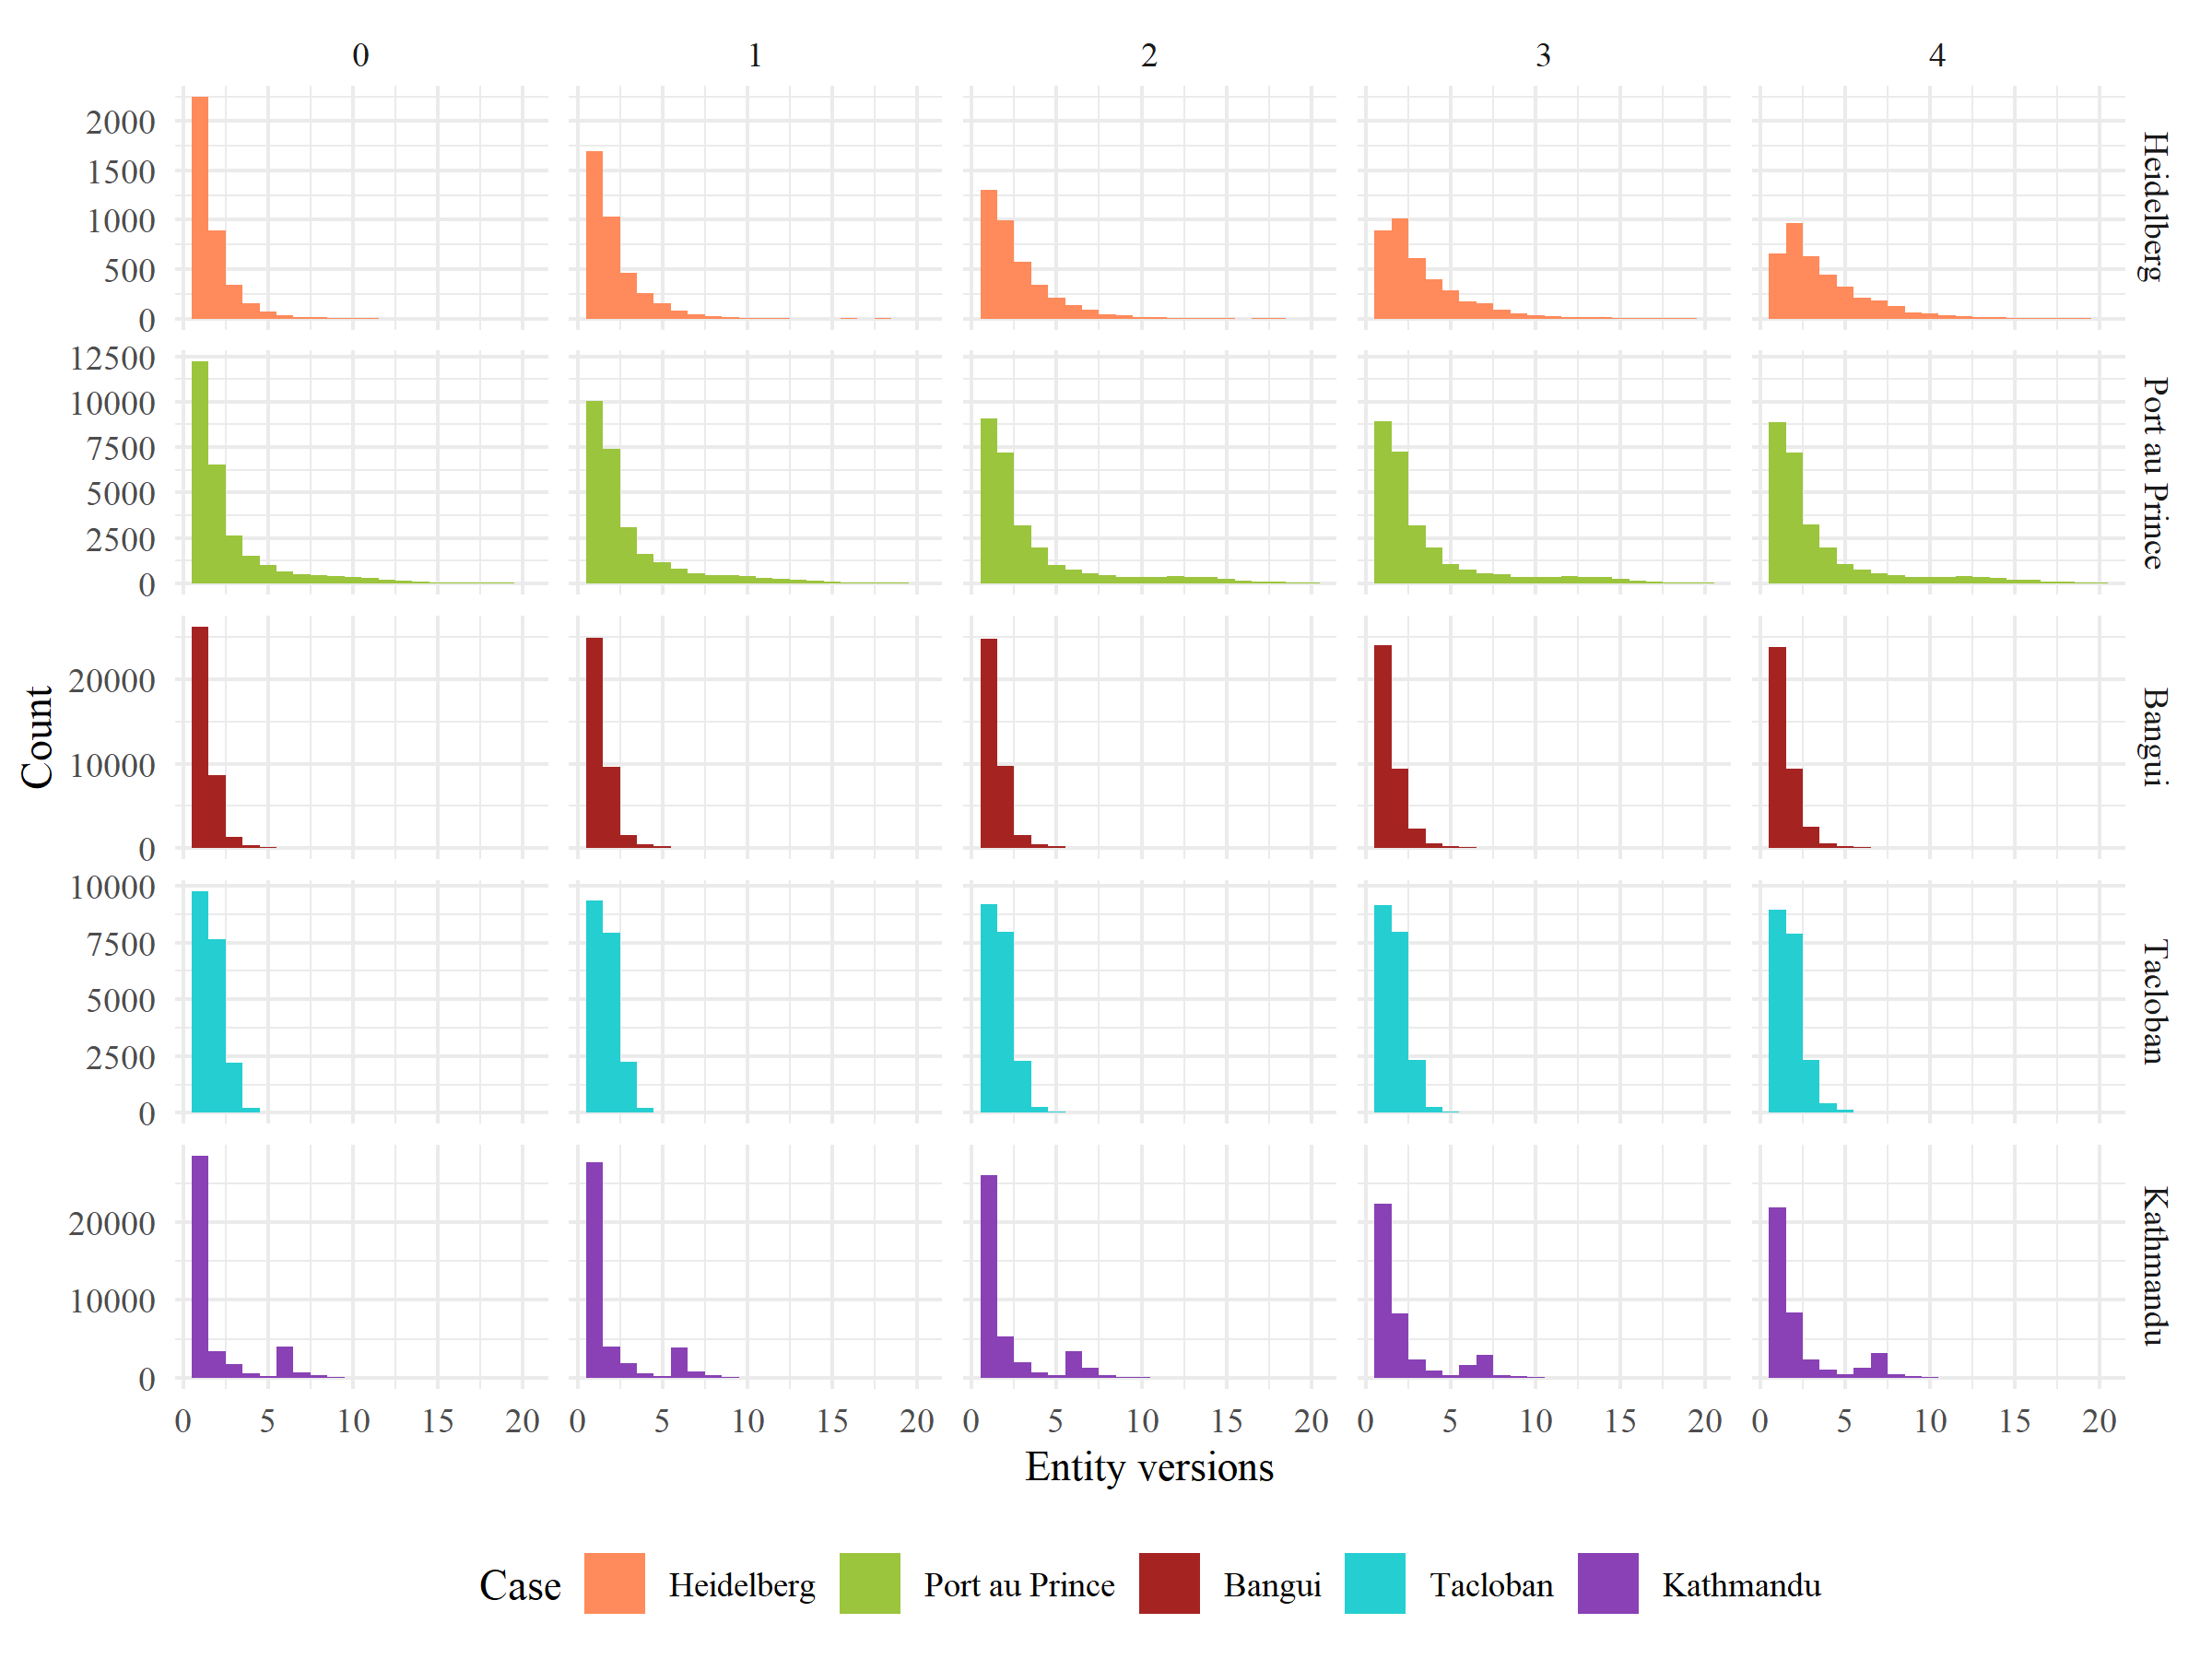
\includegraphics[width = \textwidth]{Images/facetmaint.png} %this tells latex what graphics to include. 
    \caption{Distribution of version number of OSM entities created during mapping activations, broken down across case studies and years since end of mapping activation. For visual clarity, entities with greater than 20 versions have been removed from this figure.} % this prints the caption below the figure
    \label{fig:dist} % this internally labels the figure for future referencing.
\end{figure}
%%%%%%%%%%%%%%%%%%%%%%%%%% 

In Figure \ref{fig:dist} we consider data maintenance efforts by looking at the number of versions of a given entity over time periods ranging from zero to four years following the end of each mapping activation. This figure shows the count of entities with 1-20 different versions, broken down by case study (y-axis) and time period (x-axis). Here we consider entities with only one version to have not been maintained at all. The distribution of entity versions in the 0th time period (immediately after the activation) shows that a certain degree of data modification and deletion has taken place within the mapping activation time (evidenced by the fact that there are entities with more than one version at this time). 

When comparing across case studies, we can see that the most notable changes in the distribution of entity versions over time occurs in Heidelberg. Most entities have at least two versions by the end of this four-year period, with many entities having more. In contrast, most of the entities created during the humanitarian mapping activations remain with a single version following four years. 

%%%%%%%%%%%%%%%%%%%%%%%%%% Distribution of maintenance
\begin{figure} % opens the figure environment. the '[H]' forces the image to be Here
    \centering % puts the image in the horizontal centre of the page
    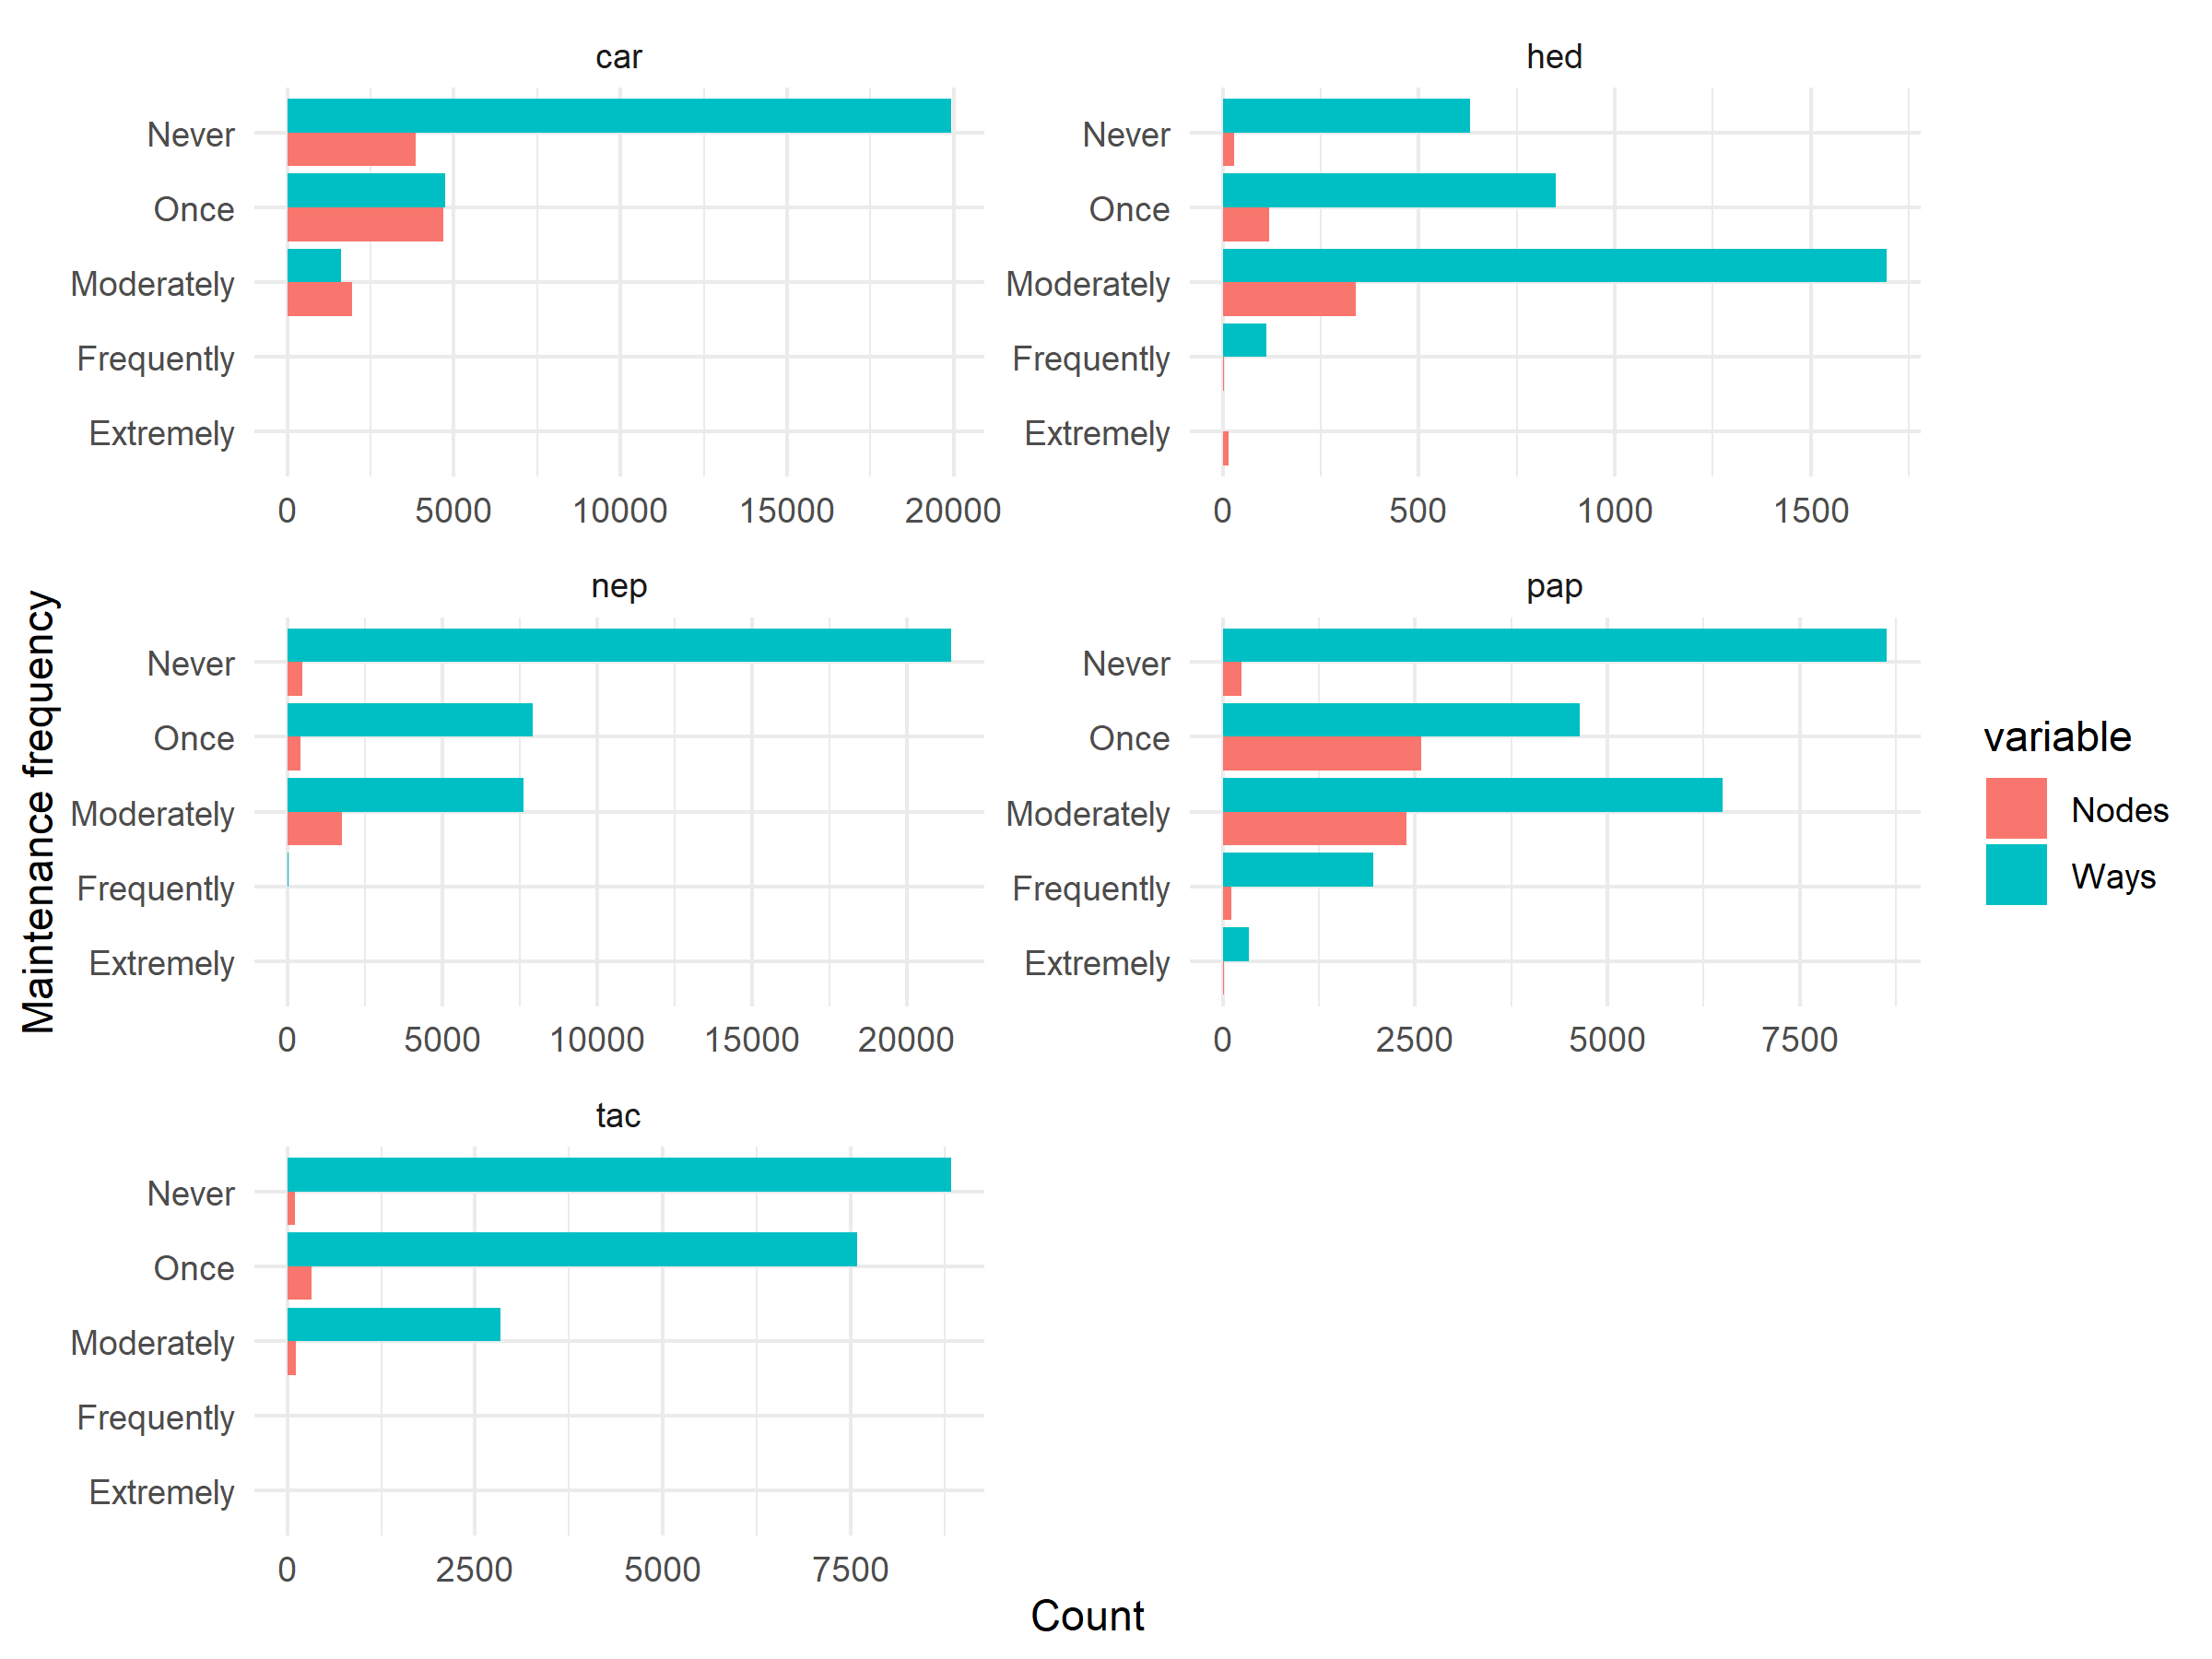
\includegraphics[width = \textwidth]{Images/types.png} %this tells latex what graphics to include. 
    \caption{Maintenance frequency of nodes and ways for each case study.} % this prints the caption below the figure
    \label{fig:types} % this internally labels the figure for future referencing.
\end{figure}
%%%%%%%%%%%%%%%%%%%%%%%%%% 

Figure \ref{fig:types} illustrates differing data maintenance frequencies between nodes and ways across all case studies. These results are calculated from the mapping activity that took place within four years following each mapping activation. As indicated previously, we see that Heidelberg is the case where, overall, entities have been updated with the greatest frequency (most have been ‘moderately’ revised). Interestingly, we see that, proportionally, nodes are maintained more frequently than ways in all case studies. Across all case studies, the majority of nodes have been maintained.  

